\chapter{一元二次方程}
    通过学习数系运算通性和等式的性质,并运用它
们解决一元一次方程和一次方程组的应用问题,使我
们初步体会到代数解法的普遍性,领略了“数系通
性”的威力.

    但是,在解决一些实际问题时,往往还可能列出
高于一次的方程式.要解决这些问题,“数系通性”、
等式的性质是不是还能发挥威力,大显神通呢?回答
是肯定的.

    本章首先学习一些有关的预备知识,然后重点讨
论最简单的高次方程——一元二次方程的解法和应
用,特别是解一元二次方程的普遍适用的方法:配方
法.

\section{平方与平方根}
\subsection{面积与平方}
    在小学算术里,已经学习过正方形的面积公式
$S=a\x a$,其中$a$是正方形的一边长,$S$是面积,也就
是:
\[S=a^2\]

这就告诉我们:一个正数的二次方,是与正方形的
面积密切相关的,这也正是$a^2$读作“$a$的平方”的道理.

    在实际问题的计算中,我们还可以有效的运用数
系运算通性(尤其是分配律),使计算达到迅速、简
捷.例如:计算边长为100.1米的正方形的面积.可
以这样进行
\begin{align*}
 S=100.1^2 &= (100+0.1)^2\\
 &= (100+0.1)(100+0.1) \tag{乘方定义}\\
 &=10000+10+10+0.01 \tag{分配律}\\
 &=10020.01\; ({\rm m}^2)  
\end{align*}

一般地,如果正方形的一边长是$(a+b)$, 那么,
它的面积就可以这样计算出来:
\begin{align*}
    S=(a+b)^2&=(a+b)\cdot (a+b) \tag{乘方定义}\\
    &=a^2+ab+ab+b^2\tag{分配律}\\
    &=a^2+2ab+b^2\tag{合并同类项}
\end{align*}

这个结果,还可以用图3.1说明:
\[\begin{split}
 & \quad \text{大正方形$ABCD$的面积$S$}\\
 &=(\text{正方形}AEMH+\text{矩形}BFME+\text{矩形}DHMG+\text{正方形}MFCG)\text{的面积}
\end{split}\]


\begin{figure}[htp]
\centering
\begin{minipage}[t]{0.48\textwidth}
\centering
\begin{tikzpicture}[scale=.7]
\draw(0,0) rectangle (6,6);
\draw(0,2)--(6,2);    
\draw(2,0)--(2,6);
\fill [pattern=north west lines] (2,0) rectangle (6,2);
\fill [pattern=north east lines] (0,2) rectangle (2,6);
\node at (1,4)[fill=white]{$ab$};
\node at (4,1)[fill=white]{$ab$};
\node at (1,1)[fill=white]{$b^2$};
\node at (4,4)[fill=white]{$a^2$};

\foreach \x/\xtext in {0/C,2/F,6/B}
{
    \node at (\x, 0) [below]{$\xtext$};
}
\foreach \x/\xtext in {0/D,2/H,6/A}
{
    \node at (\x, 6) [above]{$\xtext$};
}
\node at (0,2)[left]{$G$};
\node at (6,2)[right]{$E$};

\foreach \x/\xtext in {1/b,4/a}
{
    \node at (\x, 6) [above]{$\xtext$};
    \node at (6,\x) [right]{$\xtext$};
}

\node at (2.4,2.4){$M$};
\end{tikzpicture}
\caption{}
\end{minipage}
\begin{minipage}[t]{0.48\textwidth}
\centering
\begin{tikzpicture}[scale=.6, >=latex]
    \draw(0,0) rectangle (6,6);
    \draw(0,2)--(6,2);    
    \draw(4,0)--(4,6);
    \fill [pattern=north west lines] (0,0) rectangle (6,2);
    \fill [pattern=north east lines] (4,0) rectangle (6,6);    
    \node at (2,1)[fill=white]{$ab$};
\node at (5,4)[fill=white]{$ab$};
\node at (5,1)[fill=white]{$b^2$};
\node at (2,4)[fill=white]{$(a-b)^2$};

\foreach \x/\xtext in {0/E,4/F,6/G}
{
    \node at (\x, 0) [below]{$\xtext$};
}
\foreach \x/\xtext in {0/A,4/D,6/M}
{
    \node at (\x, 6) [above]{$\xtext$};
}
\node at (0,2)[left]{$B$};
\node at (6,2)[right]{$H$};
\node at (3.3,2.4)[right]{$C$};

\draw [|<->|] (-1,0)--node[fill=white]{$a$}(-1,6);
\draw [|<->|] (0,7)--node[fill=white]{$a$}(6,7);
\draw [|<->|] (4,-1)--node[fill=white]{$b$}(6,-1);
\draw [|<->|] (7,0)--node[fill=white]{$b$}(7,2);

\end{tikzpicture}
\caption{}
\end{minipage}
\end{figure}


由图形也能说明:
\begin{equation}
    (a+b)^2=a^2+2ab+b^2
\end{equation}

这就告诉我们:任意两个正数的和的平方,等于
这两个数的平方和,再加上这两个数乘积的2倍.

同样,如果正方形的一边长是$a-b$, 那么,它的
面积也可以作以下计算:
\[\begin{split}
  S=(a-b)^2 &= ( a-b)\cdot (a-b)\\
  &=a^2-ab-ab+b^2\\
  &=a^2-2ab+b^2
\end{split}\]



这个结果,同样可以用图3.2说明:
\[\begin{split}
 & \quad \text{大正方形$ABCD$的面积$S$}\\
 &=(\text{大正方形}AEGM-\text{矩形}BEGH-\text{矩形}FGMD+\text{正方形}CFGH)\text{的面积}
\end{split}\]

由图形,也正说明:
\begin{equation}
    (a-b)^2=a^2-2ab+b^2
\end{equation}

这又告诉我们:任意两个正数差的平方,等于这
两个数的平方和,再减去这两个数乘积的2倍.

利用公式(3.1)、(3.2)进行计算是很方便的.

\begin{example}
利用公式(3.1)或(3.2)计算:
$403^2,\quad 499^2$
\end{example}

\begin{solution}
    由公式(3.1):
    \[\begin{split}
        403^2&=(400+3)^2\\
    &=400^2+2\x400\x3+3^2\\
    &=160000+2400+9\\
    &=162409
    \end{split}\]
    
    再由公式(3.2):
    \[\begin{split}
         499^2&=(500-1)^2\\
         &=500^2-2\x500\x1+1^2\\
         &=250000-1000+1\\
         &=249001   
    \end{split}\]
\end{solution}  

不难验证,在公式(3.1)与(3.2)中,当$a,b$取任意
的两个有理数时,结论仍然是正确的.也就是说:
\textbf{任意两个有理数的和(或差)的平方,等于这两
个数的平方和,再加上(或减去)这两个数乘积的2
倍}.两公式可以合并写成:
\[(x\pm y)^2=x^2\pm 2xy+y^2\]
并分别叫做两数和(或差)的平方公式.

\begin{example}
计算:$\left(1\frac{1}{2}\right)^2,\quad (-1.99)^2,\quad \left(9\frac{7}{9}\right)^2,\quad \left(1-\frac{a}{2}\right)^2$
\end{example}

\begin{solution}
\[\begin{split}
    \left(1\frac{1}{2}\right)^2 &=\left(1+\frac{1}{2}\right)^2\\
    &=1+2\x1\x\frac{1}{2}+\frac{1}{4}=2\frac{1}{4}
\end{split}\]
\[\begin{split}
    (-1.99)^2&=(-2+0.01)^2\\
    &=4-2\x 2\x 0.01+0.0001=3.9601
\end{split}\]
\[\begin{split}
    \left(9\frac{7}{9}\right)^2&=\left(10-\frac{2}{9}\right)^2\\
    &=100-2\x 10\x \frac{2}{9}+\frac{4}{81}=\frac{7744}{81}\\
    &=95\frac{49}{81}
\end{split}\]
\[\begin{split}
    \left(1-\frac{a}{2}\right)^2&=1-2\x 1\x \frac{a}{2}+\frac{a^2}{4}\\
    &=1-a+\frac{a^2}{4}
\end{split}\]
\end{solution}

两数和(或差)的平方公式,在应用中要灵活掌
握,公式中的字母既可以是任意二个有理数.又可以
是两个算式.


\begin{example}
    利用公式展开下列各题:
$(2a+y)^2,\qquad (-3a+2x)^2$
\end{example}


\begin{solution}
\begin{enumerate}
    \item 把$2a,y$分别当作公式中的$x,y$, 因此,
\[\begin{split}
    (2a+y)^2&=(2a)^2+2\x(2a)\x y+y^2\\
&=4a^2+4ay+y^2
\end{split}\]
\item 把$-3a,2x$分别当作公式中的$x,y$, 因此,
\[\begin{split}
    (-3a+2x)^2&=(-3a)^2+2\x(-3a)\x(2x)+(2x)^2\\
    &= 9a^2-12ax+4x^2
\end{split}\]
\end{enumerate}
\end{solution}
    


\begin{example}
    展开:
    $\left(3a-\frac{1}{3}\right)^2,\qquad \left(-\frac{b}{2}-\frac{a}{2}\right)^2$
\end{example}


\begin{solution}
    \[\begin{split}
        \left(3a-\frac{1}{3}\right)^2&=(3a)^2-2\x(3a)\x\frac{1}{3}+\left(\frac{1}{3}\right)^2 \\
        &=  9a^2-2a+\frac{1}{9}
    \end{split}\]
    \[\begin{split}
        \left(-\frac{b}{2}-\frac{a}{2}\right)^2
        &=  \left(-\frac{b}{a}\right)^2-2\x\left(-\frac{b}{2}\right)\x\frac{a}{2}+\left(\frac{a}{2}\right)^2\\
        &=\frac{b^2}{4}+\frac{1}{2}ab+\frac{a^2}{4}
    \end{split}\]
\end{solution}

\begin{ex}
\begin{enumerate}
    \item 利用两数和(或差)的平方公式计算:
\begin{enumerate}
    \item $78^2,\quad 105^2,\quad 99^2,\quad 189^2,\quad 10.01^2,\quad 0.99^2$
    \item $(2+x)^2,\quad (y-3)^2,\quad (a-2x)^2,\quad \left(x+\frac{1}{2}\right)^2$ 
    \item $\left(5x+\frac{1}{2}\right)^2,\quad \left(4y-\frac{1}{3}\right)^2,\quad (2x-3y)^2,\quad \left(-\frac{a}{2}+\frac{b}{3}\right)^2$
\end{enumerate}
    
\item 填空白
\begin{enumerate}
    \item $\poly{1,2,1}=(\qquad\qquad)^2$
    \item $y^2+4y+(\qquad \qquad)=(y+2)^2$
    \item $x^2+(\qquad \qquad)+4a^2=(x+2a)^2$
    \item $a^2-6a+9=(\qquad \qquad)^2$
    \item $x^2-(\qquad \qquad)+\frac{1}{4}=\left(x-\frac{1}{2}\right)^2$
    \item $x^2+3x+(\qquad \qquad)=\left(x+\frac{3}{2}\right)^2$
    \item $4y^2-y+(\qquad \qquad)=(2y-\qquad \qquad)^2$
    \item $x^2-2x+3=(x+\qquad \qquad)^2+2$
    \item $y^2-6y+10=(y-3)^2+(\qquad \qquad)$
    \item $9x^2-12x+1=(\qquad \qquad)^2-3$
\end{enumerate}

\end{enumerate}    
\end{ex}

\subsection{平方根}
在实际问题中,我们还会经常遇到这样一类问
题:需要一块面积为9${\rm cm}^2$的正方形铁板,应该怎
样画线、下料呢?要解决这个问题,就要首先根据要
求,算出正方形的一边长,然后才能画出面积为9${\rm cm}^2$的正方形,进行剪裁而得到.

设面积为9${\rm cm}^2$的正方形一边长为$a$, 因此,问
题就是由$a^2=9$, 求出$a$的值.

显然,a可以取$-3$, 也可以取$+3$, 因为:
$(-3)^2=9,\quad (+3)^2=9$.

所以,所求正方形一边是3cm.($-3$不符合题意,舍去).
在数学上,这个问题就是:如何由一个数的二次
幂,反求出这一个数.

\begin{example}
    如果已知某些数的平方,分别为:
$$4,\quad 9,\quad 16,\quad 25,\quad 0.25,\quad 0.81,\quad \frac{64}{81},\quad 0$$
试求出相应的这些数.
\end{example}

\begin{solution}
由于:   
\[(\pm 2)^2=4,\quad  (\pm 3)^2=9,\quad (\pm 4)^2=16,\quad (\pm 5)^2=25\]
\[(\pm 0.5)^2=0.25,\quad (\pm 0.9)^2=0.81,\quad \left(\pm \frac{8}{9}\right)^2=\frac{64}{81},\quad 0^2=0 \]
因此,平方分别为$4,\; 9,\; 16,\; 25,\; 0.25,\; 0.81,\; \frac{64}{81},\; 0$的数各是
$$\pm 2,\quad \pm 3,\quad\pm 4,\quad\pm 5,\quad\pm 0.5,\quad\pm 0.9,\quad
\pm \frac{8}{9},\quad 0$$
\end{solution}

一般地说:如果一个数$x$的平方等于$a\; (a\ge 0)$, 即
$x^2=a$.那么,$x$就叫做$a$的平方根.例如:在上面例
题中,$\pm 2,\; \pm 3,\;\pm 4,\;\pm 5,\;\pm 0.5,\;\pm 0.9,\;
\pm \frac{8}{9}$以及0就分别叫做$4,\; 9,\; 16,\; 25,\; 0.25,\; 0.81,\; \frac{64}{81}$以及0的平方根.

由上例中可以看出:\textbf{正数的平方根有两个,这两
个平方根正好是互为相反数}.我们记作:$+\sqrt{a}$与
$-\sqrt{a}$.其中“$\sqrt{\quad}$”叫做\textbf{根号},$+\sqrt{a}$读作“正根
号$a$”,有时简写为$\sqrt{a}$,读作“根号$a$”;$-\sqrt{a}$
读作“负根号$a$”或“根号$a$的相反数”;有时还可以
把这两个平方根合并在一起写成:$\pm \sqrt{a}$.

\textbf{零的平方根,仍然是零},记作$\sqrt{0}=0$.

这里还应该指出:由于任何有理数(正、负和零)
的平方,都不可能是负数.也就是说,根本找不出这
样的数$x$, 能使$x^2$等于一个负数.所以,\textbf{负数的平方
根是无意义的.即:$\pm \sqrt{a}$这个符号,当$a<0$时,是
无意义的}.

求一个数的平方根的运算,叫做\textbf{开平方}运算,这
个数叫做被开方数.被开方数是负数时,平方根是无
意义的.如:$\sqrt{-2}$,$-\sqrt{-2}$都无意义.

显然,开平方运算是平方运算的逆运算.

\begin{example}
    求下列各数的平方根:$36,\quad \frac{49}{121},\quad 0.0004,\quad -25$
\end{example}

\begin{solution}
$\because\quad (\pm 6)^2=36$,

$\therefore\quad $36的平方根是$+6$与$-6$.即:$\pm\sqrt{36}=\pm 6$

$\because \quad \left(\pm \frac{7}{11}\right)^2=\frac{49}{121}$

$\therefore\quad \frac{49}{121}$的平方根是$\pm\frac{7}{11}$,即$\pm\sqrt{\frac{49}{121}}=\pm\frac{7}{11}$.

$\because\quad (\pm 0.02)^2=0.0004$,

$\therefore\quad $0.0004的平方根是$\pm 0.02$.即:$\pm\sqrt{0.0004}=\pm 0.02$

$\because\quad -25<0$, 任何数的平方,都不会等
于$-25$.

$\therefore\quad -25$的平方根是无意义的.
\end{solution}

\begin{example}
    求下列各平方根的值:
    \[\sqrt{144},\quad -\sqrt{225},\quad -\sqrt{\frac{4}{9}},\quad \sqrt{(-2)^2}   \]
\end{example}

\begin{solution}
    只要注意:“$\sqrt{\quad}$”仅表示正平方根或零,
    $-\sqrt{\quad}$”只表示负平方根,就可以由平方根的意义
得出:
\[\sqrt{144}=12,\quad -\sqrt{225}=-15,\quad -\sqrt{\frac{4}{9}}=-\frac{2}{3},\quad \sqrt{(-2)^2}=\sqrt{4}=2   \]
\end{solution}
    

也许有的同学会问:要是遇到被开方数$a$不是,
或一下子看不出是某个有理数的平方时,它是否还有
平方根呢?如果有,又怎么求呢?以下我们将以$a=2$
为例,说明$\sqrt{2}$是存在的,至于如何求出它的值,下
一段再去讨论.

要说明$\sqrt{2}$的存在问题,就是要说明:“能够找
到一个数$x$, 使
$x^2=2$”.还可以说,就是要“找出
一个面积是2的正方形来,它的边长就是所找的数
x”.也就是2的一个平方根.

我们可以这样来分析:

因为,边长为1的正方形面积是1,
边长为2的正方形面积是4.
所以,如果把正方形的边长从1逐渐加大到2的
时候,正方形的面积也应该从1逐渐加大到4.在这
个过程中,势必会经过面积正好是2的一个正方形.
可见,面积是2的正方形是存在的.实际上,我国古
代数学中,早在两三千年前就能实实在在的画出一个
面积为2的正方形来了(如图3.3).



\begin{figure}[htp]
    \begin{center}
        \begin{tikzpicture}[scale=.5]
        \draw[pattern= north east lines] (0,0) rectangle (8,8);
        \draw[fill=white] (4,0)--(8,4)--(4,8)--(0,4)--(4,0);    
        \foreach \x/\xtext in {0/B,4/F,8/C}
        {
            \node at (\x,0)[below]{$\xtext$};
        }
        \foreach \x/\xtext in {0/A,4/H,8/D}
        {
            \node at (\x,8)[above]{$\xtext$};
        }
\node at (0,4)[left]{$E$}; \node at (8,4)[right]{$G$};
\foreach \x in {2,6}
{
    \node at (\x,0)[below]{1};\node at (\x,8)[above]{1};
    \node at (0,\x)[left]{1};\node at (8,\x)[right]{1};
}
\foreach \x in {1,7}
{
    \node at (\x,\x)[fill=white] {$\tfrac{1}{2}$};
    \node at (\x,8-\x)[fill=white]{$\tfrac{1}{2}$};
}
\node at (4,4){\Large 2};
\node at (2,2)[right]{$\sqrt{2}$};  \node at (6,2)[left]{$\sqrt{2}$};
\node at (2,6)[right]{$\sqrt{2}$};   \node at (6,6)[left]{$\sqrt{2}$};
        \end{tikzpicture}
        \end{center}  
    \caption{}
\end{figure}

作图:
\begin{enumerate}
    \item 以2为边长,作正方形$ABCD$, 其面积为4.
    \item 取$ABCD$各边的中
点$E$、$F$、$G$、$H$, 并且连接$EF, FG, GH, HE$.
\end{enumerate}

可以证明$EFGH$也是一个正方形,这个小正方形正
是面积等于2的正方形.因为:
\[\text{小正方形$EFGH$的面积}=\text{大正方形$ABCD$
的面积}-4\x\text{三角形$AEH$的面积}\]
即:
\[\text{$EFGH$的面积}=4-4\x \frac{1}{2}=2\]

由此可知,面积为2的正方形的实际存在,正说
明了2的平方根是存在的.

同学们还可以进行一个实验:把图中四个小三角
形剪下来,拼在一起正好又是一个小正方形,且与图中
原有的小正方形完全相等.因而可以得出:
\[2\x \text{小正方形面积}=\text{大正方形面积}\]
因此:
\[\text{小正方形面积}=\frac{1}{2}\x \text{大正方形面积}=\frac{1}{2}\x 4=2\]
这又说明了,图中所作出来的小正方形正是面积
为2.因而,它的一边长就是2的一个平方根2.

既然$\sqrt{2}$是存在的,它能使$(\sqrt{2})^2=2$.显然,
$(-\sqrt{2})^2=2$.所以,2的平方根也应有两个$\pm \sqrt{2}$.

用类似的办法,可以说明:任一个正有理数的平
方根都是存在的.而且都有两个.同学们可以从图
3.4, 3.5中,练习说明$\sqrt{3}$,$\sqrt{7}$都是存在的.
从而$-\sqrt{3}$,$-\sqrt{7}$也应存在.因此,$3,7$同样各
有两个平方根:$\pm\sqrt{3}$,$\pm\sqrt{7}$等等.

\begin{figure}[htp]
    \centering
    \begin{minipage}[t]{0.48\textwidth}
    \centering
\begin{tikzpicture}[scale=1.5]
\draw (0,0) rectangle (1+1.414, 1+1.414);    
\draw[pattern= north east lines]  (1,0)node[below]{$F$}--(2.414,1)node[right]{$G$}--(1.414,2.414)node[above]{$H$}--(0,1.414)node[left]{$E$}--(1,0);
\node at (0,0)[below]{$B$};
\node at (2.414,0)[below]{$C$};
\node at (0,2.414)[above]{$A$};
\node at (2.414,2.414)[above]{$D$};
\node at (2.414/2,2.414/2)[fill=white]{\Large 3};
\node at (.5,0)[below]{1}; \node at (3.414/2,0)[below]{$\sqrt{2}$}; 
\node at (0,1.414+0.5)[left]{1}; \node at (0,1.414/2)[left]{$\sqrt{2}$}; 
\node at (1.414+0.5,2.414)[above]{1}; \node at (1.414/2,2.414)[above]{$\sqrt{2}$}; 
\node at (2.414, .5)[right]{1}; \node at (2.414, 3.414/2)[right]{$\sqrt{2}$}; 

\end{tikzpicture}
    \caption{}
    \end{minipage}
    \begin{minipage}[t]{0.48\textwidth}
    \centering
    \begin{tikzpicture}
\draw (0,0) rectangle (3.732, 3.732);    
\draw[pattern= north west lines]  (1.732,0)node[below]{$F$}--(3.732,1.732)node[right]{$G$}--(2,3.732)node[above]{$H$}--(0,2)node[left]{$E$}--(1.732,0);
\node at (0,0)[below]{$B$};
\node at (3.732,0)[below]{$C$};
\node at (0,3.732)[above]{$A$};
\node at (3.732,3.732)[above]{$D$};    
\node at (3.732/2,3.732/2)[fill=white]{\Large 7};

\node at (2.732,0)[below]{2}; \node at (1.732/2,0)[below]{$\sqrt{3}$}; 
\node at (0,1)[left]{2}; \node at (0,2.732)[left]{$\sqrt{3}$}; 
\node at (1,3.732)[above]{2}; \node at (2.732,3.732)[above]{$\sqrt{3}$}; 
\node at (3.732, 2.732)[right]{2}; \node at (3.732, 1.732/2)[right]{$\sqrt{3}$}; 

    \end{tikzpicture}
    \caption{}
    \end{minipage}
    \end{figure}
    
综合以上讨论,可以得出结论:

\begin{blk}{}
    \begin{itemize}
        \item 任意一个正数的平方根有两个,它们互为相反
数.

记作:$\pm \sqrt{a}\quad (a>0)$.
\item 零的平方根,仍然是零,记作:$\sqrt{0}=0$.
\item 任意一个负数的平方根无意义.
    \end{itemize}
\end{blk}

\begin{ex}
\begin{enumerate}
    \item 求下列各数的平方根:$900,\quad 
    \frac{196}{225},\quad 0.0121,\quad 4\frac{9}{4}$

\item 求下列各值:
\[-\sqrt{81},\quad \sqrt{\frac{4}{9}},\quad \sqrt{1},\quad \sqrt{0},\quad -\sqrt{0.000016}\]
\[\sqrt{\frac{1}{25}},\quad -\sqrt{7^2},\quad \sqrt{(-7)^2},\quad \left(\sqrt{4}\right)^2,\quad \left(\sqrt{-9}\right)^2\]

\item 利用所画的图3.6,说明$\sqrt{\frac{5}{2}}$是存在的.
 \end{enumerate}
\end{ex}


\begin{figure}[htp]
    \centering
    \begin{tikzpicture}[scale=2]
\draw (0,0) rectangle (2, 2);    
\draw[pattern= north west lines]  (.5,0)--(2,.5)--(1.5,2)--(0,1.5)--(.5,0);
\node at (1,1)[fill=white]{\Large $\frac{5}{2}$};
\node at (.25,0)[below]{0.5}; \node at (2.5/2,0)[below]{1.5}; 
\node at (0,3.5/2)[left]{0.5}; \node at (0,1.5/2)[left]{1.5}; 
\node at (3.5/2,2)[above]{0.5}; \node at (1.5/2,2)[above]{1.5}; 
\node at (2,.25)[right]{0.5}; \node at (2, 2.5/2)[right]{1.5}; 
    \end{tikzpicture}
    \caption{}
\end{figure}

因为一个正数$a$的正平方根$\sqrt{a}$可以理解为:
面积为$a$的正方形,边长为$\sqrt{a}$.而且知道面积较大
的正方形,边长也一定较长.所以,较大的正数,它
的正平方根也较大,而它的负平方根反而较小.即:

\begin{blk}{}
    如果$a>b>0$, 那么就有
    $$\sqrt{a}>\sqrt{b},\qquad -\sqrt{a}<-\sqrt{b}$$
\end{blk}

 
\begin{example}
比较下列各平方根的大小:
\begin{enumerate}
    \item $\sqrt{12}$ 与 $\sqrt{15}$
    \item 3 与 $\sqrt{10}$
    \item 2.1 与 $\sqrt{3}$ 与 $-\sqrt{3}$
\end{enumerate}
\end{example}

\begin{solution}
    比较平方根的大小,可以由比较被开方数的大小而决定.
\begin{enumerate}
    \item $\because\quad 12<15,\qquad \therefore\quad \sqrt{12}<\sqrt{15}$
    \item  $\because\quad 3=\sqrt{9},\; \sqrt{9}<\sqrt{10},\qquad \therefore\quad 3<\sqrt{10}$
    \item  $\because\quad 2.1=\sqrt{4.41},\;\sqrt{4.41}>\sqrt{3}>-\sqrt{3}$
    
    $\therefore\quad 2.1>\sqrt{3}>-\sqrt{3}$
\end{enumerate}

\end{solution}




\begin{example}
    试求下列各等式中的$x$、$y$值:
    \begin{enumerate}
        \item $\sqrt{x+2}=0$
        \item $\sqrt{x}+\sqrt{y-1}=0$
    \end{enumerate}
\end{example}


\begin{solution}
只要注意$\sqrt{a}$只表示正数或0.
\begin{enumerate}
    \item $\because\quad \sqrt{x+2}=0$
    
    $\therefore\quad x+2=0\qquad \therefore\quad x=-2$  
    \item $\because\quad \sqrt{x}$与$\sqrt{y-1}$表示正数或0,
    
    $\therefore\quad \sqrt{x}\ge 0, \; \sqrt{y-1}\ge 0$,因此,要使两
    部份的和为零,只有它们同时为零才行.

    $\therefore\quad\sqrt{x}=0\qquad \sqrt{y-1}=0$

    所以:$x=0,\quad y-1=0$,即$y=1$.
\end{enumerate}
\end{solution}

\begin{ex}
\begin{enumerate}
    \item 比较大小
    \begin{multicols}{2}
\begin{enumerate}
    \item $\sqrt{5}$与$\sqrt{7}$
    \item 3与$\sqrt{3}$与$-\sqrt{2}$
    \item $-\sqrt{\frac{1}{2}}$与0与$\sqrt{\frac{1}{9}}$
    \item 2与$\sqrt{4.1}$与$-2.1$与$\sqrt{\frac{20}{7}}$
\end{enumerate}
    \end{multicols}

    \item 求$x$值:
\begin{enumerate}
    \item $\sqrt{x}=0$
    \item $\sqrt{x-a}+\sqrt{b}=0$
    \item $\sqrt{x+1}+\sqrt{y-7}=0$
\end{enumerate}
\end{enumerate}
    
\end{ex}

\subsection{求一个数的平方根}
任一个正数$a$的平方根有两个:互为相反数的两
个数,零的平方根,仍是零.

我们把\textbf{正数$a$的正平方根,叫做这个数的算术平
方根},仍用记号$a$表示.

零的算术根,仍然是0,即$\sqrt{0}=0$.

任一个正方形的边长,就是其面积的算术平方
根.

要求一个正数的平方根(两个),只要求出这个
正数的算术平方根(一个)来就可以了.因为,另一
个平方根,就是算术平方根的相反数.

以下介绍两种求平方根的方法:

\subsubsection{开平方方法}
\begin{example}
    求$\sqrt{2809}$
\end{example}

\begin{solution}
    首先,应确定所求算术平方根的\textbf{位数},我们
知道:
\begin{center}
    \begin{tabular}{ll}
       $1^2=1$   &  $9^2=81$ \\
       $10^2=100$   &  $99^2=9801$ \\
       $100^2=10000$   &  $999^2=998001$ \\
       $\cdots\cdots$   &  $\cdots\cdots$ \\ 
    \end{tabular}
\end{center}

可见,
\begin{itemize}
    \item 一位数的平方是一或二位数;
    \item 两位数的平方是三或四位数;
    \item 三位数的平方是五或六位数;
    \item ……
\end{itemize}


反过来看,就有这样的规律:
\begin{itemize}
    \item 一、二位数的平方根,一定是一位数;
    \item 三、四位数的平方根,一定是二位数;
    \item 五、六位数的平方根,则必是三位数;
    \item ……
\end{itemize}

因此,如果把给出的被开方数,从个位起自右向
左每两位数字分为一段,用“'”号分开,则所分成
的“段数”,就是所求平方根应有的整数的位数.把
2809分段,得28'09.可以确定它开方后,所得平方
根是两位整数.

其次,应确定平方根最高位的数字,因为
$$50^2<2809<60^2$$
所以,$\sqrt{2809}$的最高位数字应是5(实际是50).

第三步,应确定平方根最高位数字的下一位数
字.

我们可以设为$b$, 这时,理应有:
\[\sqrt{2809}=50+b  \quad \Rightarrow\quad 2809=(50+b)^2\]
$\therefore\quad 2809=50^2+2\x 50\x b+b^2$
\begin{align}
    2809-50^2&=2\x 50\x b+b^2 \nonumber \\
    309&=(2\x 50+b)\cdot b
\end{align}
用这个等式关系,可以试商确定$b$:只要把其中的
$(2\x50+b)\cdot b$, 近似地看作$2\x50\x b$,就可以得出
\[309\approx 2\x50\x b\]
从而可以试算出$b\approx 3$.然后,再把$b\approx 3$代入关系式(3.3)
进行正式计算:
\[(2\x50+b)\cdot b=(2\x50+3)\x3=309\]
正好符合要求,$\therefore\quad b=3$ 是正确的.

归纳以上各步,可以将整个过程写成以下竖式的
形式:
\begin{center}
    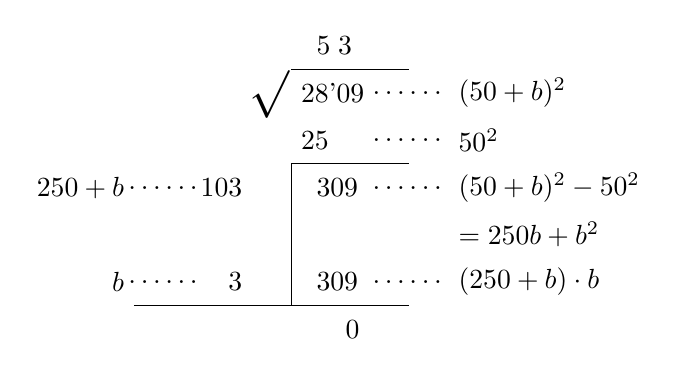
\begin{tikzpicture}[yscale=.6]
    \node at (0,2)[right]{\;\;5\;3};
\node at (0,1)[right]{28'09};  \node at (2,1)[right]{$(50+b)^2$};
\node at (0,0)[right]{25};     \node at (2,0)[right]{$50^2$};
\node at (0,-1)[right]{\;\;309};     \node at (2,-1)[right]{$(50+b)^2-50^2$};    \node at (2,-2)[right]{$=2\x 50\x b+b^2$};   
\node at (-.5,-1)[left]{103};   \node at (-2,-1)[left]{$2\x 50+b$}; 
\node at (.1,1)[left]{\LARGE $\sqrt{}$};

\node at (0,-3)[right]{\;\;309};     \node at (2,-3)[right]{$(2\x 50+b)\cdot b$};
\node at (-.5,-3)[left]{3}; \node at (-2,-3)[left]{$b$};
\node at (0,-4)[right]{\quad\; 0}; 

\draw(0,1.5)--(1.5,1.5);
\draw(0,-3.5)--(0,-.5)--(1.5,-.5);\draw(-2,-3.5)--(1.5,-3.5);

\foreach \x in {1,0,-1,-3}
{
    \node at (1.5,\x){……};
}
\foreach \x in {-1,-3}
{
    \node at (-1.6,\x){……};
}

\end{tikzpicture}
\end{center}

以上计算结果直到余0为止.表明被开方数开平
方后得到一个整数.

如果计算最后一步余数不为0时,就要给被开方
数补0,(每次补两位0).再重复以上的计算过程,
每次可得到平方根的一个小数位数字.反复进行到最
后余0时,就得到一个混合小数形式平方根.这时,
我们说被开方数是一个完全平方数.或说:开平方可
以开得尽.
\end{solution}

在更多的情形下,对一些数进行开平方运算,反
复进行下去,总也没有余0的时候.这时,我们就说
被开方数是个不完全平方数.


\begin{example}
求$\sqrt{2}$.
\end{example}

\begin{solution}
    用开平方方法算如下:
\begin{center}
    \begin{tikzpicture}[yscale=.6, >=latex]
    \node at (0,2)[right]{1.  4 \; 1\;  4……};
\node at (0,1)[right]{2.00'00'00};  
\node at (0,0)[right]{1};    
\node (A) at (0,-1)[right]{1\;00};     
\node at (.1,1)[left]{\LARGE $\sqrt{}$};
\node at (0,-2)[right]{\;\; 96};  
\node (B) at (0,-3)[right]{\quad\; 4\;00};
\node at (0,-4)[right]{\quad\; 2\;81};
\node (C) at (0,-5)[right]{\quad\; 1\;19\;00};
\node at (0,-6)[right]{\quad\; 1\;12\;96};
\node at (0,-7)[right]{\qquad\quad 6\;04};
\node at (0,-7.6)[right]{\qquad\qquad $\vdots $};
\draw(0,1.5)--(3,1.5);

\foreach \x in {-2.5,-4.5,-6.5}
{
    \draw (-0.5-\x*.15,\x)--(3,\x);
    \draw (-0.5-\x*.15,\x)--(-0.5-\x*.15,\x+2);
}

\node at (-.5,0) {$-)$};

\draw (-.5,-.5)--(3,-.5);
 
\foreach \x/\xtext in {-1/2\times 10+4=24, -3/2\times 140+1=281, -4/1 , -5/2\times 1410+4=2824, -6/4 , -2/4 }
{
   \node at (-.5-\x*0.15, \x)[left]{$\xtext$};
}

\node (D) at (5,-2){每次增补两位0} ;
\node (D1) at (5,-3){但平方根只增一位} ;

\draw [<-](A)--(D);
\draw [<-](B)--(D);
\draw [<-](C)--(D1);
\end{tikzpicture}
\end{center}


继续计算下去,总也得不到余数是0.这说明2开平
方是永远开不尽的,这是一个不完全平方数.    
\end{solution}

\begin{example}
    求$\sqrt{1650.7969}$
    \end{example}

\begin{analyze}
    遇到纯小数开平方,只是“分段定
位”与整数开平方不同,这时要以小数点为准,自左
向右每两位一段,每段就可确定平方根的一个小数
位;遇到混合小数开平方,就必须从小数点起,向左
和向右每两位一段,用“'”号分开.所分段数就可
确定平方根的整数位和小数位.以下各步骤仍与例3.10,
例3.11的方法相同.
\end{analyze}

\begin{solution}
    \begin{center}
 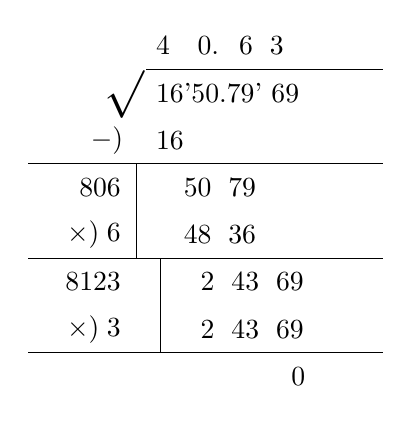
\begin{tikzpicture}[yscale=.6, >=latex]
    \node at (0,2)[right]{4\quad 0. \;6\; 3};
\node at (0,1)[right]{16'50.79' 69};  
\node at (0,0)[right]{16};    
\node  at (0,-1)[right]{\quad 50\; 79};     
\node at (.1,1)[left]{\LARGE $\sqrt{}$};
\node at (0,-2)[right]{\quad 48\; 36};  
\node   at (0,-3)[right]{\quad\; 2\; 43\; 69};
\node at (0,-4)[right]{\quad\; 2\; 43\; 69};
\node   at (0,-5)[right]{\qquad\qquad\;\; 0};
\draw(0,1.5)--(3,1.5);

\foreach \x in {-2.5,-4.5}
{
    \draw (-1.5,\x)--(3,\x);
    \draw (-0.5-\x*.15,\x)--(-0.5-\x*.15,\x+2);
}

\node at (-.5,0) {$-)$};

\draw (-1.5,-.5)--(3,-.5);
 
\foreach \x/\xtext in {-1/806 , -2/\times)\; 6  , -3/8123, -4/\times)\; 3 }
{
   \node at (-.2, \x)[left]{$\xtext$};
}

\end{tikzpicture}       
    \end{center}
\end{solution}

\begin{rmk}
这个开平方运算中,在第二位试商时不足
1,就要在平方根相应的位置“商0”,然后再继续
往下进行计算.还要注意:小数点的位置要与被开方
数的小数点对齐.
\end{rmk}

\begin{ex}
    求下列各算术平方根:
\[\sqrt{676},\qquad \sqrt{1521},\qquad \sqrt{82369},\qquad \sqrt{10309},\qquad \sqrt{4.9284}\]
\[\sqrt{9.0601},\qquad \sqrt{4901.4001},\qquad \sqrt{144.7},\qquad \sqrt{3}\]
    (要求求出两位小数).
    试总结一下开平方方法的步骤.
\end{ex}

\subsubsection{平方根表}

一个数的算术平方根,除用开平方方法可以计算
出来以外,还可以直接查《平方根表》而得到.

\begin{table}[ht]
    \centering
    \resizebox{\linewidth}{!}{%
        \begin{tabular}{|c|cccccccccc|ccccccccc|}
            \hline
            N   & 0                           & 1                          & 2     & 3     & 4     & 5     & 6     & 7     & 8     & 9     & 1 & 2 & 3 & 4 & 5 & 6 & 7 & 8 & 9 \\
            \hline
            3.5 & 1.871                       & 1.873                      & 1.876 & 1.879 & 1.881 & 1.884 & 1.887 & 1.889 & 1.892 & 1.895 & 0 & 1 & 1 & 1 & 1 & 2 & 2 & 2 & 2 \\
            3.6 & 1.897                       & 1.900                      & 1.903 & 1.905 & 1.908 & 1.910 & 1.913 & 1.916 & 1.918 & 1.921 & 0 & 1 & 1 & 1 & 1 & 2 & 2 & 2 & 2 \\
            3.7 & 1.924                       & 1.926                      & 1.929 & 1.931 & 1.934 & 1.936 & 1.939 & 1.942 & 1.944 & 1.947 & 0 & 1 & 1 & 1 & 1 & 2 & 2 & 2 & 2 \\
            3.8 & 1.949                       & 1.952                      & 1.954 & 1.957 & 1.960 & 1.962 & 1.965 & 1.967 & 1.970 & 1.972 & 0 & 1 & 1 & 1 & 1 & 2 & 2 & 2 & 2 \\
            3.9 & 1.975                       & 1.977                      & 1.980 & 1.982 & 1.985 & 1.987 & 1.990 & 1.992 & 1.995 & 1.997 & 0 & 1 & 1 & 1 & 1 & 2 & 2 & 2 & 2 \\
            4.0 & \multicolumn{10}{c|}{\dots} & \multicolumn{9}{c|}{\dots}                                                                                                     \\
            \hline
        \end{tabular}%
    }
\end{table}

这个表分两部分,标有$N$的直行(列)和横行的
数是被开方数;其余的数都是平方根数.最后一栏是
修正值.修正值表示的都是指平方根末位数字的修正
值.

在表中所查出的平方根大多数还是近似值.都是
采用四舍五入法则而得的四位数字.

平方根表中可以直接查出由1到99.99间的每一个
数的算术平方根.

例如,要查$\sqrt{3.887}$,只要首先在表里$N$所在的
列中找到被开方数的左边两位数3.8,然后再在$N$所
在的行中找到被开方数的左边第三位数字8,从第一
次找到的3.8所在的行横着看,从第二次找到的8所
在的列竖直看,交叉地方的数,就是$\sqrt{3.880}$ 的值.
再加上被开方数最末一位数字7所在列的修正值,就
可得到:
\[\sqrt{3.887}=1.970+0.002=1.972\]
又如,查$\sqrt{81.13}=9.006+0.002=9.008$. 

\begin{ex}
    查平方根表,求下列算术平方根.
\[\sqrt{1.28},\qquad \sqrt{7.320},\qquad \sqrt{66.71},\qquad \sqrt{8.247},\qquad \sqrt{91.15} \]
\end{ex}

小于1或大于100的被开方数,它的算术平
方根从表里不能直接查出来.怎么办呢?可以从分析
以下例题中,探求规律,寻找方法,设法创造条件,
利用表来查.


\begin{example}
    求出下列各平方根.并观察、总结其中有何
规律:
\begin{enumerate}
    \item $\sqrt{0.0036},\quad \sqrt{0.36},\quad \sqrt{36},\quad \sqrt{3600},\quad \sqrt{360000}$
    \item $\sqrt{0.0009},\quad \sqrt{0.09},\quad \sqrt{9},\quad \sqrt{900},\quad \sqrt{90000} $
\end{enumerate}
\end{example}

\begin{solution}
\[\begin{array}{ll}
    \sqrt{0.0036}=0.06\qquad \qquad  &  \sqrt{0.0009}=0.03 \\
     \sqrt{0.36}=0.6 &  \sqrt{0.09}=0.3\\
      \sqrt{36}=6 & \sqrt{9}=3 \\
      \sqrt{3600}=60 &  \sqrt{900}=30 \\
       \sqrt{360000}=600 &  \sqrt{90000} =300
\end{array}\]
\end{solution}

从中我们发现:当被开方数扩大(或缩小)100倍
时,它的算术平方根就相应地扩大(或缩小)10倍.
由此可以得出:\textbf{当被开方数的小数点每向右(或向左)
移动两位时,它的平方根的小数点就相应地向右(或
向左)移动一位}.

这样一来,对于大于100和小于1的被开方数,
我们就可以首先移动它的小数点位置(注意必须两位
两位地移),使它成为表内可以查到的数.

例如:
\begin{itemize}
    \item 366.2先移动小数点,成为3.662,
    \item 4733 先移动小数点,成为47.33,
    \item 37140先移动小数点,成为3.7140,
\end{itemize}

又如:
\begin{itemize}
    \item 0.1478 先移动小数点,成为14.78,
    \item 0.0536 先移动小数点,成为5.36,
    \item 0.00004先移动小数点,成为40等.
\end{itemize}

这样的向
    左或向右移动小数点,就是把被开方数缩小或扩大
    100倍、10000倍,……;
然后进行查表,得出平方根后,还需要\textbf{把查得数
的小数点再向相反的方向移动,移动的位数应是被开
方数小数点移动位数的一半}.例如:
\begin{center}
\begin{tikzpicture}[yscale=.6, >=latex]
\node at (0,0) {\Large $\because$ 查$\sqrt{3.662}=1.914$,\qquad $\therefore\; \sqrt{366.2}=19.14$};    
\draw[->,  very thick] (2.8,-.4)--(2.8,-1.5)--node[above]{左移2位}(-3,-1.5)--(-3,-.4)    ;
\draw[->, dashed,  thick] (-1.2,-.4)--(-1.2,-2.5)--node[above]{右移1位}(4.5,-2.5)--(4.5,-.4) ;
\end{tikzpicture}    
\end{center}

$\because$ 查$\sqrt{47.33}=6.880$,\qquad $\therefore\; \sqrt{4733}=68.80$

$\because$ 查$\sqrt{3.714}=1.927$,\qquad $\therefore\; \sqrt{37140}=192.7$


\begin{center}
\begin{tikzpicture}[yscale=.6, >=latex]
    \node at (0,0) {\Large $\because$ 查$\sqrt{14.78}=3.845$,\qquad $\therefore\; \sqrt{0.1478}=0.3845$};      
\draw[->,  very thick] (2,-.4)--(2,-1.5)--node[above]{右移2位}(-3,-1.5)--(-3,-.4)    ;
\draw[->, dashed,  thick] (-1.4,-.4)--(-1.4,-2.5)--node[above]{左移1位}(4.2,-2.5)--(4.2,-.4)    ;
\end{tikzpicture}
\end{center}

$\because$ 查$\sqrt{5.36}=2.315$,\qquad $\therefore\; \sqrt{0.0536}=0.2315$

$\because$ 查$\sqrt{40}=6.325$,\qquad $\therefore\; \sqrt{0.00004}=0.006325$

要注意,四位数学用表,只能查四个数码的数.
因此,若是遇到有5位以上的数字,如:$\sqrt{3.7896}$, 就
要首先用四舍五入法,将它改写为$\sqrt{3.790}$, 再去查
表.

\begin{ex}
    查平方根表,求出下列各值:
\[\sqrt{144},\quad \sqrt{297},\quad \sqrt{3756},\quad \sqrt{4444},\quad \sqrt{54542},\quad \sqrt{70107} \]
\[\sqrt{1981000},\quad \sqrt{23060000},\quad \sqrt{0.1},\quad \sqrt{0.142},\quad \sqrt{0.0787} \]
\[\sqrt{0.4333},\quad \sqrt{0.5555},\quad \sqrt{0.00063},\quad \sqrt{0.00007},\quad \sqrt{0.0000041} \]
\end{ex}

\subsection{实数}
在前面,我们用开平方的方法曾经计算过$\sqrt{2}$的
值.并指出$\sqrt{2}=1.4142\cdots$是无穷尽的,而且是永
不循环的小数.但现实又告诉我们:$\sqrt{2}$又确实存
在(面积为2的正方形的边长).

象$\sqrt{2}$这样的数,还有许多,比如:
$\sqrt{3}=1.7321\cdots$, $\sqrt{5}=2.236\cdots$, 等等.这些
数的共同特征是:\textbf{无限不循环小数}.

当然,无限不循环小数,不一定都是由开方运算
开不尽而得到的.数学中常见的还有:圆周率
$\pi=3.1415926\cdots$; $e=2.718281\cdots$; 等.它们也是\textbf{无
限不循环小数}.

可以证明这些无限不循环小数,不能化为两个整
数比$\frac{a}{b}$
的形式.因此,它们已不属于有理数的范围
了.

我们把\textbf{无限不循环小数,称为无理数}.(或称为
\textbf{非比数}).如:$\sqrt{2},\sqrt{3},e,\pi$都是无理数.

\textbf{有理数与无理数统称为实数.}

全体实数组成的集合,叫做实数集合,简称\textbf{实数
集},记作:集合$\mathbb{R}$.

实数集,是可以用来度量长度,面积的数集,其
详细内容、运算将在高中学习.这里只简略地指出:
在实数范围内,也有以下概念:

如果用字母$a$表示任一个实数,则$-a$就是它的相
反数.即$(+a)+(-a)=(-a)+(+a)=0$.

例如:$\sqrt{2}$与$-\sqrt{2}$互为相反数,即$\sqrt{2}+\left(-\sqrt{2}\right)=0$.

如果字母$b$表示任一个非零实数,
则$\frac{1}{b}$
就是它的
倒数,即$b\x\frac{1}{b}=1$
例如:$\sqrt{3}$与$\frac{1}{\sqrt{3}}$
互为倒数,即$\sqrt{3}\x \frac{1}{\sqrt{3}}=1$.

任一实数$x$的绝对值的意义,与有理数时的意义
相同.即
\[|x|=\begin{cases}
    x, & x>0\\
    0, & x=0\\
    -x, & x<0\\  
\end{cases}\]

例如:$|\sqrt{3}|=\sqrt{3}$, $|0|=0$, $|-e|=e$.

显然,任一实数$x$的绝对值,总是非负数.
即$|x|\ge 0$.

归纳我们已经学习过的数,可列成下表:

\begin{center}
\begin{tikzpicture}
\node  at (0,0)[right]{实数};
\node  at (1,1)[right]{有理数};
\node at (1,-1)[right]{无理数};
\node at (2.5,1.5)[right]{正有理数};
\node  at (2.5,1)[right]{零};
\node  at (2.5,.5)[right]{负有理数};
\node  at (2.5,-.5)[right]{正无理数};
\node  at (2.5,-1.5)[right]{负无理数};
\node  at (4.25,1.75)[right]{正整数(自然数)};
\node  at (4.25,1.25)[right]{正分数(小数)};
\node  at (4.25,.75)[right]{负整数};
\node  at (4.25,.25)[right]{负分数(负小数)};

 \draw[decorate,decoration=brace] (1,-1) -- (1,1);
 \draw[decorate,decoration=brace] (2.5,.5) -- (2.5,1.5);
 \draw[decorate,decoration=brace] (2.5,-1.5) -- (2.5,-.5);
 \draw[decorate,decoration=brace] (4.3,1.1) -- (4.3,1.9);
 \draw[decorate,decoration=brace] (4.3,.1) -- (4.3,.9);
\end{tikzpicture}
\end{center}



\begin{ex}
\begin{enumerate}
    \item  指出下列实数中,哪些是有理数,哪些是无理数:
    \[3.1416,\quad -0.2,\quad \sqrt{0.09},\quad -\sqrt{7},\quad \pi,\quad 0.\dot{0}\dot{1},\quad 0.010010001\cdots\]
    \item 指出下列各实数的相反数,倒数及绝对值都是什么:
    \[-1.41,\quad \sqrt{3},\quad -\pi,\quad -\sqrt{5},\quad 0,\quad \frac{1}{\sqrt{2}},\quad -0.\dot{2}\dot{3},\quad 2.40\dot{1},\quad -\sqrt{16}\]
\end{enumerate}   
\end{ex}

\section*{习题3.1}
\addcontentsline{toc}{subsection}{习题3.1}
\begin{enumerate}
    \item 试用两数和或差的平方公式,计算:
\[\left(2\frac{1}{2}\right)^2,\qquad 9.997^2,\qquad 401^2\]
    \item 利用公式,把下列各式展开:
\begin{multicols}{2}
\begin{enumerate}
    \item $\left(2a+\frac{1}{2}\right)^2$
    \item $\left(2x+\frac{1}{2}y\right)^2$
    \item $(4y-1)^2$
    \item $(2m-2n)^2$
    \item $\left(\frac{x+y}{2}\right)^2$
    \item $\left(\frac{a-2b}{3}\right)^2$
\end{enumerate}
\end{multicols}
    \item 把下列各式中的空白填上适当的数:
\begin{enumerate}
    \item $x^2+x+(\qquad\qquad  )=(x+\qquad\qquad  )^2$
    \item $2x^2+4x+(\qquad\qquad   )=2(x+\qquad\qquad  )^2$
    \item $-m^2+(\qquad\qquad   )-64=-(m-\qquad\qquad  )^2$
    \item $4y^2-(\qquad\qquad  )+1=(2y-1)^2$
    \item $-3x^3-3x-(\qquad\qquad  )=-3\left(x+\frac{1}{2}\right)^2$
    \item $x^2+6x-1=(x+3)^2-(\qquad\qquad   )$
\end{enumerate}
    \item \begin{enumerate}
        \item 一个正数的平方等于289, 求这个正数.
        \item 一个数的平方等于361, 求这个数.
        \item 一个负数的平方等于196, 求这个负数.
    \end{enumerate}
    
\item 由$m^2=n^2$而得出$m=n$正确吗?为什么?
\item 求下列各平方根:
\[\sqrt{36},\quad -\sqrt{81},\quad \sqrt{\frac{9}{16}},\quad \sqrt{1},\quad -\sqrt{7^2},\quad -\sqrt{(-4)^2}\]
\[\sqrt{0},\quad \sqrt{(-\sqrt{4})^2},\quad -\sqrt{\left(-\frac{1}{361}\right)^2}\]
\item 求下列各数的算术平方根.
\[900,\quad 121,\quad 1,\quad 0,\quad \frac{196}{256},\quad (-25)^2\]

\item 比较下列各平方根的大小:
\begin{enumerate}
    \item $\sqrt{3},\qquad \sqrt{3.1},\qquad 2$
    \item $-\sqrt{7},\qquad \sqrt{6},\qquad \sqrt{\frac{1}{6}}$
    \item $15,\qquad \sqrt{220},\qquad -\sqrt{250},\qquad -\sqrt{225}$
\end{enumerate}

\item 如果$\sqrt{a+3}+\sqrt{b}=0$, 试求$a$与$b$的值.
\item 七块同样大小的正方形面积之和是343平方米,求每块
正方形的一边长是多少?
\item 用开平方方法,求下列各算术根:
\[\sqrt{9025},\qquad \sqrt{2116},\qquad \sqrt{3969},\qquad \sqrt{50625},\qquad \sqrt{269361}\]
\[\sqrt{0.4489},\qquad \sqrt{0.00080089},\qquad \sqrt{8114.4064}\]
\item 查平方根表,求下列各数的算术平方根:
\[99.23,\quad 9.123,\quad 4.017,\quad 17.536,\quad 174,\quad 1981,\quad 2006,\quad 
75693,\quad 1001230\]
\[0.101,\quad 0.07864,\quad 0.00043,\quad 0.000801,\quad 
0.000006123\]
\item 什么是无理数?什么是实数?
\item 要使一个正整数乘以60以后,得出一个完全平方
数,问:这一个正整数最小是几才行?这个完全平方数是
几?它的算术平方根是几?
\end{enumerate}

\section{平方根的运算}
本节仅就算术平方根进行讨论,其中所提到的平
方根,就是指$\sqrt{a},\quad (a\ge 0)$.

\subsection{算术平方根的性质}

\begin{blk}{性质1}
    算术平方根的平方,等于被开方数,即:
$$\left(\sqrt{a}\right)^2=a\qquad (a\ge 0)$$
\end{blk}

这只要由平方根的意义就可看出.

例如:$(\sqrt{3})^2=3,\quad (\sqrt{7})^2=7,\quad \left(\sqrt{\frac{2}{5}}\right)^2=\frac{2}{5}$
等.

\begin{blk}{性质2}
    一个数的平方的算术平方根,等于这个
数的绝对值.即
\[\sqrt{x^2}=|x|=\begin{cases}
    x,& x>0\\
    0, &x=0\\
    -x, & x<0
\end{cases}\]
\end{blk}

这个性质可以这样来分析、说明:

首先,任一个数 $x$ 的平方,必是非负数.即:
$x^2\ge 0$,因而算术平方根$\sqrt{x^2}$是有意义的.

其次,当$x$为正数或零时,由平方根的定义,显
然有$\sqrt{x^2}=x,\quad (x>0)$.

例如:
$\sqrt{7^2}=7,\quad\sqrt{\left(\frac{3}{4}\right)^2}=\frac{3}{4},\quad \sqrt{0^2}=0$等.


再次,当$x$为负数时,仍有$x^2>0$, 因而,算术平
方根$\sqrt{x^2}=-x$. (特别注意,$\because\; x<0, \therefore\; -x>0$).

例如:$\sqrt{(-5)^2}=\sqrt{25}=-(-5)=5$; 
$\sqrt{(-0.4)^2}=\sqrt{0.16}=-(-0.4)=0.4$等.

综合以上,可以断定:

对任一数$x$来说,都有下式成立:
\[\sqrt{x^2}=|x|=\begin{cases}
    x,& x>0\\
    0, &x=0\\
    -x, & x<0
\end{cases}\]


\begin{example}
    求出下列算术平方根:
\[ \sqrt{(-0.12)^2},\qquad \sqrt{6\x 14\x 21},\qquad \sqrt{(-3)^6} \]
\end{example}

\begin{solution}
\begin{enumerate}
    \item $ \sqrt{(-0.12)^2}=-(-0.12)=0.12$
    \item $\sqrt{6\x 14\x 21}=\sqrt{2\x3\x2\x7\x3\x7}=\sqrt{(2\x3\x7)^2}=42$
    \item $\sqrt{(-3)^6}=\sqrt{[(-3)^3]^2}=-(-3)^3=27$
\end{enumerate}
\end{solution}

\begin{example}
    化简:
\begin{multicols}{2}
\begin{enumerate}
    \item $\sqrt{(a-1)^{2}}\quad (a>1)$
    \item $\sqrt{(b-5)^{2}}\quad (b<5)$
    \item $\sqrt{(c-7)^{2}}\quad (c=7)$
    \item $\sqrt{(10-x)^{2}}$
\end{enumerate}
\end{multicols}
\end{example}

\begin{solution}
\begin{enumerate}
    \item $\because a>1 \quad \therefore a-1>0$
    
    $\therefore \quad \sqrt{(a-1)^{2}}=|a-1|=a-1$
    \item   $\because b<5 \quad \therefore \quad b-5<0$
    
    $\therefore \quad \sqrt{(b-5)^{2}}=|b-5|=-(b-5)=5-b$

    \item  $\because c=7, \quad \therefore \quad c-7=0$
    
    $\therefore \quad \sqrt{(c-7)^{2}}=|c-7|=0$.

    \item  $\because x$ 是任意数, $\therefore 10-x$ 就可能为正或0或
    负, 因此:
\[\sqrt{(10-x)^2}=|10-x|=\begin{cases}
    10-x,& \text{当$10-x>0$ 即$x<10$时}\\
    0,&\text{当$10-x=0$ 即$x=10$时}\\
    x-10,&\text{当$10-x<0$ 即$x>10$时}\\
\end{cases} \]
\end{enumerate}
\end{solution}

\begin{ex}
    利用算术根的性质,化简:
\begin{enumerate}
    \item $(\sqrt{0.7})^{2},\qquad \sqrt{(-5)^{2}}, \qquad(\sqrt{-5})^{2},\qquad -\sqrt{5^{2}},\qquad (-\sqrt{5})^{2}$
    \item $\sqrt{7^{2} \times 9^{2}},\qquad \sqrt{8 \times 18 \times 9},\qquad \sqrt{12 \times 15 \times 20}$
    \item $\sqrt{(2-x)^{2}}\quad (x>2),\qquad \sqrt{(5+x)^{2}},\qquad \sqrt{(5-x)^{2}}$
    \item  $\sqrt{a^{8}},\qquad \sqrt{(\sqrt{2}-2)^{2}},\qquad \sqrt{(1-\sqrt{3})^{2}},\qquad \sqrt{(\sqrt{2}-\sqrt{5})^{2}}$
    \item 如果 $\sqrt{(x)^{2}}+\sqrt{(y-1)^{2}}=0$, 你能知道 $x$、$y$ 各是什么值吗?
\end{enumerate}
\end{ex}
    
\subsection{算术平方根的乘、除运算}
首先来计算平方根$\sqrt{25}\cdot \sqrt{9}$与$\sqrt{25\x9}$的值:
$$\sqrt{25}\cdot \sqrt{9}=5\x3=15\qquad \sqrt{25\x9}=\sqrt{225}=15$$
可见,$\sqrt{25}\cdot \sqrt{9}=\sqrt{25\x9}$.

一般地说:如果$a\ge 0$, $b\ge 0$, 那么,就有
$\sqrt{a}\cdot \sqrt{b}=\sqrt{ab}$成立.

这就是说:\textbf{二数算术平方根的积等于这二数积的
算术平方根}.即
\[\sqrt{a}\cdot \sqrt{b}=\sqrt{ab}\qquad (a\ge 0,\; b\ge 0)\]

\begin{note}
    $\because\quad$已知$a\ge 0$, $b\ge 0$,应有$ab\ge 0$.
$\therefore\quad \sqrt{a},\sqrt{b}$都是算术平方根,应
有$\sqrt{a}\ge 0$, $\sqrt{b}\ge 0$.因而$(\sqrt{a}\cdot \sqrt{b})\ge 0$.

根据乘积的乘方运算律可知:
\begin{align*}
    (\sqrt{a}\cdot \sqrt{b})^2 &= (\sqrt{a})^2\cdot (\sqrt{b})^2\\
    &=a\cdot b=ab \tag{算术平方根的性质}
\end{align*}
$\therefore\quad \left(\sqrt{a}\cdot \sqrt{b}\right)^2=ab$

又由于$\sqrt{a}\cdot\sqrt{b}\ge 0$, $ab\ge0$, 因此,利用平方
根的定义就可以得出:
\[\sqrt{a}\cdot\sqrt{b}=\sqrt{ab}\]
\end{note}

\begin{example}
化简下列各平方根,使被开方数的每一个因
数的指数都小于2:
\begin{multicols}{2}
\begin{enumerate}
    \item $\sqrt{4^2\x3}$
    \item $\sqrt{100a}\quad (a\ge 0)$
    \item $\sqrt{125x^3}$
    \item $\sqrt{a^2b}\quad (a\ge 0\; b\ge 0)$
\end{enumerate}
\end{multicols}
\end{example}

\begin{solution}
\begin{enumerate}
\item $\sqrt{4^2\x3}=\sqrt{4^2}\cdot \sqrt{3}=4\sqrt{3}$
    \item $\sqrt{100a}=\sqrt{100}\cdot \sqrt{a}=10\sqrt{a} $
    \item $\sqrt{125x^3}=\sqrt{5^2\cdot x^2\cdot 5\cdot x}=\sqrt{5^2}\cdot \sqrt{x^2}\cdot \sqrt{5x}=5x\sqrt{5x}$
    \item $\sqrt{a^2b}=\sqrt{a^2}\cdot \sqrt{b}=a\sqrt{b} $
\end{enumerate}
\end{solution}

由这个例题说明,利用算术平方根的乘法法则,
可以把被开方数中的“完全平方因数”,用它的算术
平方根代替,而移到根号外边.这种变形,通常叫做
把根号内的因数开方后移到根号外边,从而可以化简
根式.

有时候,还可以反过来把根号外边的因数平方
后,移到根号里边去,以利于计算和化简.
    
\begin{example}
    比较下列各数的大小:
\begin{enumerate}
    \item $2\sqrt{5},\qquad \sqrt{17}$
   \item $a\sqrt{b},\qquad \sqrt{1+a^2b}\quad  (a\ge0,\; b\ge0)$
\end{enumerate}
\end{example}

\begin{solution}
    \begin{multicols}{2}
        \begin{enumerate}
    \item $\because\quad 2\sqrt{5}=\sqrt{4}\cdot \sqrt{5}=\sqrt{20}$
    
    且$\sqrt{20}>\sqrt{17}$.
   
   $\therefore\quad  2\sqrt{5}>\sqrt{17}$

    \item $\because\quad a\sqrt{b}=\sqrt{a^2}\cdot \sqrt{b}=\sqrt{a^2b}$
    
    且$\sqrt{a^2b}<\sqrt{1+a^2b}$.

   $\therefore\quad  a\sqrt{b}<\sqrt{1+a^2b}$
   
   $(a\ge 0,\; b\ge 0)$
\end{enumerate}  
    \end{multicols}
  
\end{solution}

\begin{example}
    计算:
$\sqrt{6}\cdot \sqrt{27},\qquad a\sqrt{b}\cdot b\cdot \sqrt{ab}\quad  (a\ge0,\; b\ge0)$
\end{example}

\begin{solution}
\begin{enumerate}
    \item $\sqrt{6}\cdot \sqrt{27}=\sqrt{2\x3\x3^3}=\sqrt{2}\cdot \sqrt{3^4}=9\sqrt{2}$
    \item $a\sqrt{b}\cdot b \sqrt{ab}=ab\sqrt{ab^2}=ab\cdot b\sqrt{a}=ab^2\sqrt{a}$
\end{enumerate}
\end{solution}

\begin{ex}
\begin{enumerate}
    \item 把被开方数中的因数尽量移到根号外,使各因数的指数都
    小于2:
 \[   \sqrt{5\x7^2},\quad \sqrt{48},\quad \sqrt{50},\quad \sqrt{36ab^2}\; (b\ge 0),\quad  \sqrt{24a^2}\; (a<0)\]
    \item 把根号外边的因数移到根号里边去:
 \[   2\sqrt{3},\qquad 3\sqrt{6},\qquad 5\sqrt{a},\qquad a\sqrt{2}\;(a\ge 0),\qquad b\sqrt{a}\; (b<0)\]
    \item 计算:$\sqrt{10}\cdot \sqrt{125},\qquad \sqrt{7}\cdot \sqrt{14},\qquad a\sqrt{a}\cdot b\sqrt{a}$
\end{enumerate}
\end{ex}

再来计算$\frac{\sqrt{16}}{\sqrt{49}}$与$\sqrt{\frac{16}{49}}$的值:
\[\frac{\sqrt{16}}{\sqrt{49}}=\frac{4}{7},\qquad \sqrt{\frac{16}{49}}=\frac{4}{7}  \]
可见,$\frac{\sqrt{16}}{\sqrt{49}}=\sqrt{\frac{16}{49}}$.

一般地说,如果$a\ge 0$, $b>0$, 那么,就有$\frac{\sqrt{a}}{\sqrt{b}}=\sqrt{\frac{a}{b}}$成立.

这就是说:\textbf{二数算术平方根的商,等于这二数商
的算术平方根}.即
\[\frac{\sqrt{a}}{\sqrt{b}}=\sqrt{\frac{a}{b}}\qquad (a\ge 0,\; b>0)\]

\begin{note}
    $\because\quad a\ge 0, \; b>0$,因而$\frac{a}{b}\ge 0$

    $\therefore\quad \sqrt{a},\; \sqrt{b}$都是算术平方根,应有:$\sqrt{a}\ge 0,\; \sqrt{b}>0$,因而:$\frac{\sqrt{a}}{\sqrt{b}}\ge 0$.

    根据商的乘方运算律可知:
    \begin{align*}
\left(\frac{\sqrt{a}}{\sqrt{b}}\right)^2&=\frac{(\sqrt{a})^2}{(\sqrt{b})^2}\\
&=\frac{a}{b}\tag{算术平方根的性质}     
    \end{align*}
$\therefore\quad \left(\frac{\sqrt{a}}{\sqrt{b}}\right)^2=\frac{a}{b}$

又由于$\frac{\sqrt{a}}{\sqrt{b}}\ge 0$,$\frac{a}{b}\ge 0$,因此,由平方根的定义
就可以得出:
\[\frac{\sqrt{a}}{\sqrt{b}}=\sqrt{\frac{a}{b}}\]

\end{note}

\begin{example}
    计算:$\frac{\sqrt{125}}{\sqrt{5}},\qquad \sqrt{\frac{8}{49}}$
\end{example}


\begin{solution}
    $\frac{\sqrt{125}}{\sqrt{5}}=\sqrt{\frac{125}{5}}=\sqrt{25}=5$

    $\sqrt{\frac{8}{49}}=\frac{\sqrt{8}}{\sqrt{49}}=\frac{2\sqrt{2}}{7}$
\end{solution}

在算术平方根的运算中,常常需要通过一些变形
把分母中的根号化去或把根号中的分母化去,这叫做
\textbf{分母有理化}.


\begin{example}
    化简下列各平方根,使分母有理化:
    \[ \sqrt{\frac{5}{7}},\qquad \frac{2}{\sqrt{3}} \]
\end{example}


\begin{solution}
\begin{align*}
    \sqrt{\frac{5}{7}}&=\sqrt{\frac{5\x 7}{7\x 7}}\tag{分数的基本性质}\\
    &=\frac{\sqrt{35}}{7}
\end{align*}
\begin{align*}
    \frac{2}{\sqrt{3}} &=\frac{2\x \sqrt{3}}{\sqrt{3}\cdot \sqrt{3}} \tag{分数的基本性质}\\
    &=\frac{2\sqrt{3}}{3}
\end{align*}
\end{solution}

一般地:
\begin{blk}{}
    \[\begin{split}
     \frac{\sqrt{a}}{\sqrt{b}}&=\frac{\sqrt{a}\cdot \sqrt{b}}{\sqrt{b}\cdot \sqrt{b}}=\frac{\sqrt{ab}}{b}\\
     \sqrt{\frac{a}{b}}&=\sqrt{\frac{a\x b}{b\x b}}=\frac{\sqrt{ab}}{b}\quad 
        (a\ge 0,\; b>0)
    \end{split}\]
\end{blk}



\begin{example}
    把下列平方根的分母有理化:
    \[\sqrt{2\frac{1}{2}},\quad \frac{3}{2\sqrt{5}},\quad \frac{5}{\sqrt{40}},\quad \sqrt{\frac{25}{3a}},\quad \frac{1}{\sqrt{2}\cdot \sqrt{3}}\]
\end{example}


\begin{solution}
\[\begin{split}
    \sqrt{2\frac{1}{2}} &=\sqrt{\frac{5}{2}}=\sqrt{\frac{5\x 2}{2\x 2}}=\frac{\sqrt{10}}{2}\\
    \frac{3}{2\sqrt{5}}&=\frac{3\sqrt{5}}{2\sqrt{5}\cdot \sqrt{5}}=\frac{3\sqrt{5}}{10}\\
    \frac{5}{\sqrt{40}}&=\frac{5}{2\sqrt{10}}=\frac{5\sqrt{10}}{2\x \sqrt{10}\cdot \sqrt{10}}=\frac{5\sqrt{10}}{20}=\frac{\sqrt{10}}{4}\\
    \sqrt{\frac{25}{3a}}&=\frac{5}{\sqrt{3a}}=\frac{5\sqrt{3a}}{3a}\\
    \frac{1}{\sqrt{2}\cdot \sqrt{3}}&= \frac{1}{\sqrt{6}}=\frac{\sqrt{6}}{6}   
\end{split}\]    
\end{solution}

\begin{ex}
\begin{enumerate}
    \item 将下列各平方根的分母有理化:
    \[\sqrt{\frac{7}{36}},\qquad \sqrt{\frac{25}{4a^2}}\; (a>0),\qquad \sqrt{\frac{2}{9a}},\qquad 2\sqrt{\frac{1}{8}}\]
    \[ 6\sqrt{\frac{1}{3}},\qquad \frac{\sqrt{3}}{\sqrt{2}\cdot \sqrt{6}},\qquad \frac{\sqrt{2}}{\sqrt{5}\cdot \sqrt{6}}  \]
    \item 化简:(就是使被开方数的每一个因数的指数都小于
    2,使分母有理化)
\[\sqrt{75},\quad 7\sqrt{\frac{5}{7}},\quad 4\sqrt{\frac{1}{3}},\quad \sqrt{45},\quad \sqrt{0.2},\quad \sqrt{2\frac{1}{8}},\quad \sqrt{\frac{1}{2}} \]
    \item 先化简,再比较以下各组数的大小:
    \[\sqrt{24}\text{ 与 }\sqrt{54},\qquad \sqrt{\frac{7}{12}}\text{ 与 }\sqrt{\frac{28}{243}}\]
\end{enumerate}
  \end{ex}  

  在今后的平方根运算中,如果没有特别声明,运
  算结果都要求符合两个条件:
  \begin{enumerate}
      \item 被开方数的每个因数
  的指数小于2;
  \item 分母有理化.
  \end{enumerate}
符合这两个条件的平
  方根,称为\textbf{最简平方根}.


\begin{ex}
    把下列各平方根,化为最简平方根:
\[\sqrt{180},\qquad \sqrt{200},\qquad \sqrt{\frac{63}{2a}},\qquad \sqrt{7\frac{1}{2}b^2}\; (b\ge 0) \]
\end{ex}

\subsection{算术平方根的加、减运算}
对于算术平方根的加、减运算,只要首先把各个
平方根化为最简平方根,再利用数系运算的通性,就
可以进行同一算术平方根的加法和减法运算.
\begin{example}
计算:
$\sqrt{12}+\sqrt{75}-\sqrt{48}-\frac{1}{\sqrt{3}}-\frac{1}{2\sqrt{3}}$
\end{example}

\begin{solution}
\begin{align*}
    &\quad \sqrt{12}+\sqrt{75}-\sqrt{48}-\frac{1}{\sqrt{3}}-\frac{1}{2\sqrt{3}}\\
    &=2\sqrt{3}+5\sqrt{3}-4\sqrt{3}-\frac{\sqrt{3}}{3}-\frac{\sqrt{3}}{6} \tag{化简}\\
    &=\left(2+5-4-\frac{1}{3}-\frac{1}{6}\right)\sqrt{3} \tag{分配律}\\
    &=2\frac{1}{2}\x \sqrt{3}=\frac{5\sqrt{3}}{2}
\end{align*}
\end{solution}

\begin{example}
    计算:$\sqrt{27}+\sqrt{2}+5\sqrt{5}+4\sqrt{3}-\sqrt{3}-\sqrt{20}$
\end{example}

\begin{solution}
\begin{align*}
    &\quad \sqrt{27}+\sqrt{2}+5\sqrt{5}+4\sqrt{3}-\sqrt{3}-\sqrt{20}\\
    &=3\sqrt{3}+\sqrt{2}+5\sqrt{5}+4\sqrt{3}-\sqrt{3}-2\sqrt{5} \tag{化简}\\
    &=\left(3\sqrt{3}+4\sqrt{3}-\sqrt{3}\right)+\sqrt{2}+\left(5\sqrt{5}-2\sqrt{5}\right) \tag{交换、结合律}\\
    &=(3+4-1)\sqrt{3}+\sqrt{2}+(5-2)\sqrt{5} \tag{分配律}\\
    &=6\sqrt{3}+\sqrt{2}+3\sqrt{5}
\end{align*}
\end{solution}

\begin{example}
计算:$\sqrt{0.5}-2\sqrt{\frac{1}{3}}-\sqrt{\frac{1}{8}}+\sqrt{48}$
\end{example}

\begin{solution}
\begin{align*}
&\quad \sqrt{0.5}-2\sqrt{\frac{1}{3}}-\sqrt{\frac{1}{8}}+\sqrt{48}\\
&=\frac{1}{2}\sqrt{2}-\frac{2}{3}\sqrt{3}-\frac{1}{4}\sqrt{2}+4\sqrt{3}\\
&=\left(\frac{1}{2}-\frac{1}{4}\right)\sqrt{2}+\left(4-\frac{2}{3}\right)\sqrt{3}\\
&=\frac{1}{4}\sqrt{2}+\frac{10}{3}\sqrt{3}    
\end{align*}   
\end{solution}  


\begin{example}
    计算:$\left(5\sqrt{12}-12\sqrt{3}\right)\cdot \sqrt{6}$
\end{example}

\begin{solution}
解法1:
\begin{align*}
   \left(5\sqrt{12}-12\sqrt{3}\right)\cdot \sqrt{6}
&=\left(5\x 2\sqrt{3}-12\sqrt{3}\right)\cdot \sqrt{6} \tag{化简根式}\\
&=\left(10\sqrt{3}-12\sqrt{3}\right)\cdot \sqrt{6}\\
&=-2\sqrt{3}\cdot \sqrt{6}\tag{平方根减法}\\
&=-2\sqrt{3\x 6}=-2\x 3\sqrt{2}\\
&=-6\sqrt{2} \tag{平方根乘法}
\end{align*}
解法2:
\begin{align*}
 \left(5\sqrt{12}-12\sqrt{3}\right)\cdot \sqrt{6}
    &=5\sqrt{12}\x \sqrt{6}-12\sqrt{3}\x \sqrt{6} \tag{分配律}\\
    &=5\sqrt{12\x 6}-12\sqrt{3\x 6}\tag{平方根乘法}\\
    &=30\sqrt{2}-36\sqrt{2} \tag{化简}\\
    &=-6\sqrt{2}  \tag{平方根减法}
\end{align*}
\end{solution}

\begin{ex}
\begin{enumerate}
    \item (口答)$5\sqrt{2}+3\sqrt{2}$, $7\sqrt{3}+\sqrt{3}$, $2\sqrt{5}-3\sqrt{5}$, $\sqrt{4}+\sqrt{5}$是否等于$\sqrt{4+5}$, 为什么?

    \item 计算:
    \[\sqrt{3}\x \sqrt{2},\qquad \sqrt{6}\x \sqrt{2},\qquad \sqrt{\frac{1}{2}}\x \sqrt{2}\]
    \[3\sqrt{28}-4\sqrt{7},\quad 3\sqrt{24}-\sqrt{\frac{3}{2}},\quad 4\sqrt{2}+2\sqrt{3}-5\sqrt{2}+\sqrt{3}-5\sqrt{3}\]

    \item 计算:
    \[\sqrt{10a}\cdot \sqrt{5a},\quad \sqrt{18}\div \sqrt{6},\quad \sqrt{5}\left(\sqrt{10}-1\right),\quad \sqrt{96}\div \sqrt{3}\x \sqrt{2}\]
    \item 计算:
    \begin{enumerate}
        \item $\left(4\sqrt{27}-7\sqrt{12}\right)\div \sqrt{3}$
        \item $\left(\sqrt{\frac{1}{2}}-2\sqrt{\frac{1}{8}}+2\sqrt{0.5}\right)\x \sqrt{8}$
    \end{enumerate}
\end{enumerate}
\end{ex}

\section*{习题3.2}
\addcontentsline{toc}{subsection}{习题3.2}
\begin{enumerate}
    \item 求下列各式的值:
\[\left(\sqrt{\frac{1}{2}}\right)^2,\qquad \sqrt{(-5)^2},\qquad \sqrt{\frac{9}{16}},\qquad -\sqrt{17^2\x 8^2}  \]
\[\sqrt{17^2-8^2},\qquad \sqrt{121\x 169},\qquad \sqrt{256\x 225},\qquad \sqrt{17^2}-\sqrt{8^2}\]

\item 计算下列各式:
\begin{enumerate}
    \item $\sqrt{(a-1)^2},\qquad \sqrt{(2-b)^2},\qquad \left(\sqrt{1-\sqrt{2}}\right)^2$
    \item $\sqrt{\left(\sqrt{2}-1\right)^2}-\sqrt{\left(1-\sqrt{2}\right)^2},\qquad \sqrt{\left(\sqrt{3}-\sqrt{2}\right)^2}+\sqrt{\left(1-\sqrt{2}\right)^2}$
\end{enumerate}

\item 下列计算是否正确?为什么?
\begin{enumerate}
    \item $-2\sqrt{3}=\sqrt{(-2)^2\cdot 3}=\sqrt{12}=2\sqrt{3}$
    \item $\sqrt{-4}\cdot \sqrt{-9}=\sqrt{(-4)\x(-9)}=\sqrt{36}=6$
    \item $\sqrt{4^2+9^2}=\sqrt{4^2}+\sqrt{9^2}=4+9=13$
\end{enumerate}

\item 化简:
\begin{enumerate}
    \item $\sqrt{108},\qquad \sqrt{105},\qquad \sqrt{98},\qquad \sqrt{63},\qquad \sqrt{720},\qquad \sqrt{686}$
    \item $\sqrt{\frac{1}{7}},\qquad \sqrt{4\frac{1}{2}},\qquad 2\sqrt{\frac{3}{2}},\qquad \frac{\sqrt{7}}{\sqrt{5}},\qquad \frac{\sqrt{15}}{\sqrt{7}\cdot \sqrt{5}}$
\end{enumerate}

\item 化简:将被开方数中的因数移到根号外
\begin{enumerate}
    \item $\sqrt{1000a^2}\;\; (a>0),\qquad \sqrt{325ab^2}\;\; (b<0)$
    \item $\sqrt{0.4m^2}\;\; \text{($m$为任意有理数)},\qquad \sqrt{96x^2}\;\;\text{($x$为有理数)}$
\end{enumerate}

\item 计算下列各式:
\begin{multicols}{2}
\begin{enumerate}
    \item $\sqrt{\frac{16}{7}}\x \sqrt{7}$
    \item $\sqrt{54}\div \left(-\sqrt{6}\right)$
    \item $\sqrt{0.6}\x \sqrt{2\frac{3}{5}}$
    \item $12\sqrt{2}\div 2\sqrt{3}$
    \item $\sqrt{27}\x 3\sqrt{12}\x \frac{5}{8}\sqrt{3}$
    \item $8\sqrt{\frac{2}{7}}\div 5\sqrt{1\frac{1}{7}}$
    \item $\sqrt{96}\div 2\sqrt{3}\x \sqrt{2}$
    \item $5\sqrt{180}\div 2\sqrt{5}\div \sqrt{3}$
\end{enumerate}
\end{multicols}

\item 在下列平方根中,把根号外的因数移到根号里边去:
\begin{enumerate}
    \item $7\sqrt{2},\qquad a\sqrt{2b}\quad (a>0)$
    \item $-4\sqrt{3},\qquad b\sqrt{2}\quad (b<0)$
\end{enumerate}

\item 有理化分母:
\begin{enumerate}
    \item $\sqrt{\frac{3}{7}},\qquad \frac{\sqrt{5}}{\sqrt{3}},\qquad \frac{\sqrt{12}}{\sqrt{3}},\qquad \sqrt{\frac{7}{6}}$
    \item $\sqrt{1\frac{2}{11}},\qquad \sqrt{\frac{a}{5}},\qquad \sqrt{\frac{2}{a}},\qquad \frac{\sqrt{m}}{\sqrt{2b}} $
\end{enumerate}

\item 计算:
\begin{enumerate}
    \item $3\sqrt{8}-2\sqrt{32}$
    \item $\sqrt{96}-3\sqrt{24}+\sqrt{54}$
    \item $5\sqrt{63}+5\sqrt{7}-4\sqrt{28}$
    \item $\sqrt{75}+\sqrt{\frac{1}{3}}-\sqrt{48}$
    \item $3\sqrt{0.2}+4\sqrt{125}+\sqrt{\frac{1}{27}}-\sqrt{75}$
    \item $\sqrt{24}-\left(\sqrt{\frac{1}{2}}+2\sqrt{\frac{2}{3}}\right)-\left(\sqrt{\frac{1}{8}}-\sqrt{6}\right)$
\end{enumerate}

\item 计算:
\begin{enumerate}
    \item $\sqrt{2}(1+\sqrt{2})$
    \item $(\sqrt{10}-1)\cdot \sqrt{5}$
    \item $\sqrt{5}(2\sqrt{45}-\sqrt{15})$
    \item $(\sqrt{5}+2\sqrt{0.2})\cdot \sqrt{5}$
    \item $\sqrt{18}\left(\sqrt{2}-4\sqrt{\frac{1}{2}}\right)$
    \item $2\sqrt{3}\left(\sqrt{12}-\sqrt{6}+2\sqrt{27}\right)$
    \item $\left(\sqrt{\frac{1}{3}}+\sqrt{3}\right)\cdot \left(\sqrt{27}-\sqrt{\frac{1}{27}}\right)$
    \item $(\sqrt{2}+\sqrt{3})(\sqrt{2}-\sqrt{3})+1$
    \item $\sqrt{(\sqrt{10}-4)^2}+\sqrt{(4+\sqrt{10})^2}-\sqrt{\frac{1}{8}}\x \sqrt{2}$
\end{enumerate}

\item \begin{enumerate}
    \item 已知$p=1, \; q=-20$,试求$-\frac{p}{2}-\frac{1}{2}\sqrt{p^2-4q^2}$的值.
    \item 已知$a=-\sqrt{2},\; b=\sqrt{3}$,试求$\frac{1}{a}+\frac{1}{b}$的值. 
\end{enumerate}

\item  \begin{enumerate}
    \item 如果$x,y$都是非负数,且$\sqrt{x}+\sqrt{y}=0$, 试求
$x,y$的值.
\item 如果$\sqrt{a^2}+\sqrt{b^2}=0$, 试求$a,b$的值.
\item 如果$\sqrt{x+1}+\sqrt{y-3}=0$, 试求$x,y$的值.
\item 如果$\sqrt{x+y-6}+\sqrt{x-y-2}=0$, 试求$x,y$的
值.
\item 如果
$(x-y)^2+\sqrt{x+y-7}=0$, 试求 $x,y$的
值.
\end{enumerate}

\end{enumerate}

\section{一元二次方程及其解法}
\subsection{一元二次方程}
首先考虑一个应用问题:

要在操场上画出一块面积是32${\rm m}^2$的长方形,
并且要求它的长比宽多4m.问:这个长方形的长和
宽各取多少m?(如图
3.7)
\begin{figure}[htp]
    \centering
    \begin{tikzpicture}
\draw[pattern=north east lines] (0,0) rectangle (4,2);
\node at (2,0)[below]{$x+4$};
\node at (0,1)[left]{$x$};
\node at (2,1) [fill=white]{$32{\rm m}^2$};
    \end{tikzpicture}
    \caption{}
\end{figure}


用代数解法解这个
问题:

设 这个长方形的宽取$x$m,则它的长就应取$(x+4)$m,由题意可以
得出:
\[x(x+4)=32\]

去括号,得$x^2+4x=32$.

移项,得 $x^2+4x-32=0$.

由此得到的这种方程,其特点是:各项的最高次
数是2.

我们把\textbf{只含一个未知数、分母不含未知数,且各项
的最高次数是2的方程,叫做一元二次方程}.

例如:$x^2-9=0$, $2y^2-3y+1=0$, $3x^2-2x=0$,
$x^2+2x=5$, $-x^2-2=5x$等都是一元二次方程.

显然,任何一个一元二次方程,经过变形、整理,
都可以化成下面的标准形式:
\[ax^2+bx+c=0\quad (a\ne 0)\]
其中,$ax^2$叫\textbf{二次项},$a(\ne 0)$是\textbf{二次项系数};$bx$叫\textbf{一
次项},$b$(可取任何实数)是\textbf{一次项系数};$c$(可取任
意实数)是\textbf{常数项}.
\begin{itemize}
    \item 当$b\ne 0,\; c\ne 0$时,方程$ax^2+bx+c=0\quad (a\ne 0)$叫做\textbf{一般的}一元二次方程;
    \item 当$b=0$或$c=0$或$b=c=0$时,方程
$ax^2+c=0\quad (a\ne 0)$或$ax^2+bx=0\quad (a\ne 0)$或$ax^2=0\quad (a\ne 
0)$都叫做\textbf{特殊的}一元二次方程.
\end{itemize}

\begin{ex}
\begin{enumerate}
    \item 
    下列方程中,哪些是一元二次方程?如果是,写出它的二
    次项、一次项和常数项.
    \begin{multicols}{2}
        \begin{enumerate}
       \item $3x^2+4x=5$
       \item $-2x^2-3x+4=0$
       \item $-3x^2+36x-\sqrt{5}=0$
       \item  $\sqrt{5}x^2+\sqrt{3}x-3=0$
           \item  $x^2=3$
       \item  $7x^2=0$
           \item  $ -8x=7x^2$
           \item  $2x^2+1=0$
       \item  $\sqrt{7}x^2=1$ 
       \item  $3x^2+x-3=3x^2-1$
   \end{enumerate}
    \end{multicols}
   
   \item 把下列各方程整理成标准形式$ax^2+bx+c=0$, 并且使二次
    项系数都是正数,最后再指出$a,b,c$各是什么值?
    \begin{multicols}{2}
  \begin{enumerate}
    \item  $x^2-3=5$
    \item $4x(2-3x)=x-6$
    \item $(3x-5)(4-x)=0$
    \item $\sqrt{6}y(y+\sqrt{3})+\sqrt{2}=y$
    \item $6x-5=(2x-3)^2$ 
    \item $-x^2+8=2\sqrt{2}x$
        \item $(x-3)^2+7=(2x+1)^2$
        \item $(1+m)x- (m-1)x-x^2=m$
\end{enumerate}      
    \end{multicols}

    \item 适当引入一个未知数,根据以下问题列出方程式,并化成
    标准形式:
    \begin{enumerate}
        \item 两数的差是8, 积是48, 求两数.
        \item 两个连续的偶数之积是24, 求这两偶数.
        \item 一个两位数等于它的个位数字的平方,假若个位数字
    比十位数字大3, 试求这个两位数.
    \end{enumerate}
\item 试试看:求出下列方程的解
\[4x^2=0,\qquad  x^2-9=0,\qquad 2x^2-18=0\]
\end{enumerate}    
\end{ex}

\subsection{特殊的一元二次方程的解法}
\subsubsection{$ax^2=0$的解法}
由于$a\ne 0$, 因而,直接运用等式的性质,就可以
把原方程化为:$x^2=0$.

显然,这一方程的解(或根)就是0, 我们写成
$x=0$, 即解集为$\{0\}$.

\subsubsection{$ax^2+c=0\; (a\ne 0)$的解法}

对于特殊的一元二次方程$ax^2+c=0\; (a\ne 0)$, 可
以首先进行移项,除以$a$, 变形为:
\[x^2=-\frac{c}{a}\]
然后利用平方根的意义就可以求出这个方程的解(或
根)来.

\begin{example}
    解下列各方程:
\begin{multicols}{2}
\begin{enumerate}
    \item $5x^2-4=0$
    \item $-7x^2+7=0$
    \item $-3x^2=0$
    \item $2x^2+5=0$
\end{enumerate}
\end{multicols}
\end{example}

\begin{solution}
\begin{enumerate}
    \item 
    \begin{align*}
        5x^2-4&=0\\
        5x^2&=4\tag{移项}\\
        x^2&=\frac{4}{5} \tag{两边除以5}\\
    \end{align*}

    由平方根的意义可知:$x=\pm\sqrt{\frac{4}{5}}$,即:
\[ x_1=\frac{2}{5}\sqrt{5},\qquad x_2=-\frac{2}{5}\sqrt{5} \]
所以,原方程的解集是$\left\{\frac{2}{5}\sqrt{5},\; -\frac{2}{5}\sqrt{5}\right\}$.

\item \begin{align*}
    -7x^2+7&=0\\
    -7x^2&=-7\tag{移项变号}\\
    x^2&=1\tag{两边除以$-7$}\\
    x&=\pm 1 \tag{平方根的意义}
\end{align*}
即:$x_1=1,\quad x_2=-1$

所以,原方程的解集是$\{1,-1\}$.

\item \begin{align*}
    -3x^2&=0\\
    x^2&=0 \tag{两边除以$-3$}\\
    x&=0
\end{align*}
所以,原方程的解集是$\{0\}$.

\item \begin{align*}
    2x^2+5&=0\\
2x^2&=-5  \tag{移项变号}\\
x^2&=-\frac{5}{2} \tag{两边除以2}
\end{align*}
由于任何实数的平方,都不可能是负数,所以,
原方程没有实数根,这时,我们就说,这个方程的解
集是空集,记作$\emptyset$.
\end{enumerate}
\end{solution}

\begin{rmk}
    空集就是不包含任何实数的集合,要注意与
集合$\{0\}$是根本不同的.
\end{rmk}

通过以上例题,可以归纳出:
方程$ax^2+c=0\; (a\ne 0)$的解法步骤是:
\begin{blk}{}
\begin{enumerate}[I. ]
    \item 把原方程变形为:
    $$x^2=-\frac{c}{a}$$
    \item 根据平方根的意义,得出:
    \begin{enumerate}[1.]
        \item 当$-\frac{c}{a}>0$时,$x=\pm\sqrt{-\frac{c}{a}}$

    原方程的解集是$\left\{\sqrt{-\frac{c}{a}}, \; -\sqrt{-\frac{c}{a}}\right\}$
    \item 当$-\frac{c}{a}=0$时,$x=0$.
    原方程的解集是$\{0\}$.
    \item 当$-\frac{c}{a}<0$时,原方程没有实
    数根,即解集是空集$\emptyset$.
    \end{enumerate}
\end{enumerate}
\end{blk}

其中,当$-\frac{c}{a}=0$时,由$x^2=0$得出$x=0$, 我们为了
统一和方便,常常也看成“两个相同的根”,并叫做
原方程的二重根.但写成解集时,仍记作$\{0\}$,而不
写成$\{0,\; 0\}$.

\begin{ex}
    解下列方程:
\begin{multicols}{2}
\begin{enumerate}
    \item $9x^2=0$
    \item $25x^2-9=0$
    \item $-256x^2+144=0$ 
    \item $5x^2-7x-7=3x^2-7x+1$
    \item $2x^2=3$
    \item $3x^2+2=0$
    \item $(x-1)^2=4$
    \item $(x+1)^2=1$
\end{enumerate}
\end{multicols}
\end{ex}


\begin{example}
    解下列方程:
    \[(1-x)^2=9,\qquad 4(1+2x)^2=49\]
\end{example}

\begin{analyze}
    如果把方程中括号内的部分,看成一个整
体,那么就可以先求出这一个整体的值,然后再去求
出其中的未知数$x$的值.
\end{analyze}

\begin{solution}
\begin{enumerate}
    \item \begin{align*}
        (1-x)^2&=9\\
        (1-x)&=\pm 3 \tag{平方根的意义}
    \end{align*}
    即:    $1-x=+3$或    $1-x=-3$

    因而,$x=-2$ 或    $x=4$

 $\therefore\quad $   原方程的解集是$\{-2,4\}$.
    \item \begin{align*}
        4(1+2x)^2&=49\\
        (1+2x)^2&=\frac{49}{4}  \tag{两边除以4}\\
        1+2x&=\pm\frac{7}{2} \tag{平方根的意义}
    \end{align*}
    即:    $1+2x=+\frac{7}{2}$或    $1+2x=-\frac{7}{2}$

    因而,$x=\frac{5}{4}$ 或    $x=-\frac{9}{4}$   

    $\therefore\quad $   原方程的解集是$\left\{\frac{5}{4},\; -\frac{9}{4}\right\}$.

\end{enumerate} 
\end{solution}

由例3.27, 我们又可以归纳出:如果遇到$a(x+m)^2
+c=0$的一元二次方程,那么可以把$(x+m)$看成一
个整体,先求出$(x+m)=\pm\sqrt{-\frac{c}{a}}\quad \left(-\frac{c}{a}\ge 0\right)$
再进一步求出$x=-m\pm\sqrt{-\frac{c}{a}}$.

\begin{ex}
解下列方程:
\begin{multicols}{2}
    \begin{enumerate}
\item $(x-2)^{2}=16$
\item $(5-2 x)^{2}=4$
\item $9(50-x)^{2}=36$
\item $\frac{1}{3}(2 x-3)^{2}=25$
\item $125=5\left(x+\frac{1}{2}\right)^{2}$
\item $\frac{1}{6}(\sqrt{2} x+1)^{2}=2$
    \end{enumerate}
\end{multicols}
\end{ex}

\subsubsection{$ax^2+bx=0\; (a\ne 0)$的解法}
对于方程$ax^2+bx=0\; (a\ne 0)$, 可以先运用数系运
算通性中的分配律,把它变形为
\[(ax+b)x=0\]
然后,再利用零的运算特性,就可以得出:
\[ax+b=0\qquad  \text{或}\qquad x=0\]
这是因为:如果两个因数的乘积为0, 那么,这两个
因数中至少有一个是0.

因而,就可以进一步解出$x$的值来.

\begin{example}
    解方程 $x^2-4x=0$.    
\end{example}

\begin{solution}
    \begin{align*}
        x^2-4x&=0\\
        (x-4)x&=0\tag{分配律}\\
    \end{align*}
\[x-4=0\qquad \text{或}\qquad x=0\]
即: $x_1=4,\quad x_2=0$.

$\therefore\quad $原方程的解集是$\{4,\; 0\}$.
\end{solution}



\begin{example}
    解方程
$5x^2+3x=0$.
\end{example}

\begin{solution}
\begin{align*}
    5x^2+3x&=0\\
    (5x+3)x&=0
\end{align*}  
因而,$5x+3=0\qquad \text{或}\qquad x=0$

即:$x_1=-\frac{3}{5},\qquad x_2=0$

$\therefore\quad $原方程的解集是$\left\{-\frac{3}{5},\; 0\right\}$.
\end{solution}

由此,可归纳出:
方程$ax^2+bx=0\; (a\ne 0)$的解法步骤是:

\begin{blk}{}
\begin{enumerate}[I. ]
    \item 利用分配律变形为
    $$(ax+b)x=0$$
    \item 由零的运算特性可知
    $$ax+b=0\qquad  \text{或}\qquad x=0$$
    \item 原方程的解为
    $$x_1=-\frac{b}{a},\qquad x_2=0$$
    即解集是$\left\{-\frac{b}{a},\; 0\right\}$.
\end{enumerate}
\end{blk}

这里要指出,解方程$ax^2+bx=0$的过程,就是把
它转化为解两个一元一次方程,其转化方法,就是利
用数系运算通性,把方程左边化成两个因数的乘积形
式,这种把高次方程转化为低次方程;把新问题转化
为旧问题的解题思想是很重要的,必须很好掌握.

从这里还可以看出,方程$ax^2+bx=0\; (a\ne 0)$总
有一个根是0, 也就是说,\textbf{常数项$c=0$的一元二次方
程,必有一个根是零}.

\begin{ex}
\begin{enumerate}
    \item 解下列方程:
\begin{multicols}{2}
    \begin{enumerate}
    \item $x^{2}-5 x=0$
    \item $3 x-x^{2}=0$
    \item $4 x^{2}+6 x=0$
    \item $\frac{2}{5} x=-3 x^{2}$
    \item $x^{2}+\frac{1}{7} x=0$
    \item $x^{2}+\sqrt{2} x=0$
    \item $\sqrt{5} x=7 x^{2}$
    \item  $\sqrt{2} x^{2}-\sqrt{3} x=0$
    \item $\frac{\sqrt{2}}{2} x^{2}+1=1-\sqrt{2} x$
\end{enumerate}
\end{multicols}
\item 把下列方程中括号内的部分,看为一个整体,先求出它的
值,然后再求解:
\begin{multicols}{2}
\begin{enumerate}
    \item $(x+1)^{2}-3(x+1)=0$
    \item $(x-2)^{2}+\frac{1}{2} x-1=0$
    \item $3(3-5 x)^{2}=2(3-5 x)$
    \item $2(x+\sqrt{2})^{2}-x-\sqrt{2}=0$
\end{enumerate}
\end{multicols}
\end{enumerate}
\end{ex}

\begin{example}
解方程 $x^2-6x=0$
\end{example}

\begin{analyze}
    除用上述方法解这个特殊的一元二次方
程外,还可以利用等式性质,把它设法转化成$(x\pm 
m)^2=n$的形式,先求出整体$(x\pm m)$, 进而求出$x$的
值.
\end{analyze}

\begin{solution}
\begin{align*}
    x^2-6x&=0\\
    x^2-6x+9&=9 \tag{两边加上9}\\
    (x-3)^2&=9\\
    x-3&=\pm 3  \tag{平方根的意义}
\end{align*}    
即:$x-3=+3\quad \text{或}\quad x-3=-3$

$\because\quad x_1=6,\qquad x_2=0$

所以,原方程的解集为$\{6,0\}$.
\end{solution}

\begin{ex}
    用例3.30的方法,解下列方程:
\begin{multicols}{2}
\begin{enumerate}
    \item $x^2+4x=0$
    \item  $x^2-2\sqrt{2}x=0$
    \item $-2x^2=3x$
    \item  $5x^2-4x=0$  
\end{enumerate}   
\end{multicols}
\end{ex}

\subsection{一般的一元二次方程的解法——配方法}
对于一般一元二次方程$ax^2+bx+c=0\; (a\ne 0)$,
我们将先从本章一开始所提出的应用问题入手,利用
图形直观地说明“配方法”的想法和解决问题的具体
做法.从而归纳出它的一般解法来.

由应用题所列出的方程是:$x^2+4x=32$. 其中$x$
是所求长方形的宽,32是长方形的面积.如图3.8
所示,这个长方形可以理解为:是由一个边长为$x$的
正方形与一个边长为$x, 4$的小长方形组合而成的.

这时,我们可以如图3.9所示,把$4\x x$的小长
方形平分为两个$2\x x$的更小长方形,再把其中带阴影
的一个移至正方形$x\x x$的下方.这样,原来长方形就
变成了Г形,但面积仍为32${\rm m}^2$.
\begin{figure}[htp]
\centering
\begin{minipage}[t]{0.48\textwidth}
\centering
\begin{tikzpicture}
    \draw (0,0) rectangle (5,3);
    \draw [dashed] (3,0)--(3,3);
    \node at (0,1.5) [left] {$x$};
    \node at (2.5,3) [above] {$x+4$};
    \node at (1.5,1.5) {\Large $x^2$};
    \node at (4,1.5) {\Large $4x$};
    \node at (3,.5) {32${\rm m}^2$};
    \end{tikzpicture}
\caption{}
\end{minipage}
\begin{minipage}[t]{0.48\textwidth}
\centering
\begin{tikzpicture}
    \draw (0,0) rectangle (5,3);
    \draw (3,0)--(3,3);
\draw[dashed, pattern=north east lines] (0,0) rectangle (3,-1);
\fill[pattern=north east lines] (4,0) rectangle (5,3);
\node at (1.5,1.5)[fill=white] {\Large $x^2$};
\node at (3.5,1.5)[fill=white]  {\Large $2x$};
\node at (4.5,1.5)[fill=white]  {\Large $2x$};
\node at (1.5,-.5)[fill=white]  {\Large $2x$};
\draw [dashed](4,0)--(4,3);
\draw [dashed](0,0)--(0,-1)--(3,-1)--(3,0);
\end{tikzpicture}
\caption{}
\end{minipage}
\end{figure}

如果我们把右下方补上一
个边长为2的小正方形,如
图3.10所示,那么,就可以
得到一个边长为$(x+2)$的大正
方形.这个正方形的面积比原
来的长方形面积多了$2^2=4$.
\begin{figure}[htp]
    \centering
    \begin{tikzpicture}
        \draw (0,0) rectangle (4,4);
    \draw (0,1)--(4,1);
    \draw (3,0)--(3,4);
    \fill [pattern=crosshatch] (3,0) rectangle (4,1);
    \node at (1.5,.5)[fill=white] {\Large $2x$};
    \node at (1.5,2.5)[fill=white]  {\Large $x^2$};
    \node at (3.5,2.5)[fill=white]  {\Large $2x$};
    \node at (3.5,.5)[fill=white]  { $2^2$};
    
    \end{tikzpicture}
    \caption{}
\end{figure}


也就是说,由原来所列的方程式$x^2+4x=32$, 就
变形成为:
\[\begin{split}
    x^2+4x+2^2&=32+2^2\\
    (x+2)^2&=36\\
    x+2&=\pm 6
\end{split}\]
即$x+2=+6\quad \text{或}\quad x+2=-6$

$\therefore\quad x_1=4,\quad x_2=-8$

显然,$x=-8$不符合题意,应舍去.

所以,长方形的宽为4m,长为8m.

通过解决这个应用问题,启发我们:对一元二次
方程,可以配成完全平方后,再去求解.上例中,通
过画图直观了解到,对于二次项系数是一的一元二次
方程要配成完全平方,只要利用等式性质,方程两边
同时加上\textbf{一次项系数一半的平方数},就可以了.

\begin{example}
    用配成完全平方的方法,解方程:
\[x^2+3x=40,\qquad 2x^2+3x-5=0 \]
\end{example}

\begin{solution}
\begin{enumerate}
    \item $x^2+3x=40$的两边同加一次项系数3的一半的平方数$\left(\frac{3}{2}\right)^2$,就得到:
\begin{align*}
    x^2+3x+ \left(\frac{3}{2}\right)^2&=40+\left(\frac{3}{2}\right)^2\\
    \left(x+\frac{3}{2}\right)^2&=\frac{169}{4}\\
    x+\frac{3}{2}&=\pm\frac{13}{2}  \tag{平方根的定义}
\end{align*}
即:$x+\frac{3}{2}=+\frac{13}{2}\quad \text{或}\quad x+\frac{3}{2}=-\frac{13}{2}$

$\therefore\quad x_1=5,\qquad x_2=-8$

$\therefore\quad $原方程的解集是$\{5,\;-8\}$.
\item 先将二次项系数化简成为1, 并将方程写成
$x^2+px+q=0$的形式.两边同除以2, 得
\[x^2+\frac{3}{2}x-\frac{5}{2}=0 \]
其次,就可按1题的解法去求解:
\begin{align*}
    x^2+\frac{3}{2}x&=\frac{5}{2}\tag{移项}\\
    x^2+\frac{3}{2}x+\left(\frac{3}{4}\right)^2&=\frac{5}{2}+\left(\frac{3}{4}\right)^2 \tag{配方}\\
    \left(x+\frac{3}{4}\right)^2&=\frac{49}{16}\\
    x+\frac{3}{4}&=\pm\frac{7}{4} \tag{平方根意义}
\end{align*}
即:$x+\frac{3}{4}=+\frac{7}{4} \quad \text{或}\quad x+\frac{3}{4}=-\frac{7}{4} $

$\therefore\quad x_1=1,\qquad x_2=-\frac{5}{2}$

$\therefore\quad $原方程的解集是$\left\{1,\;-\frac{5}{2}\right\}$.
\end{enumerate}
\end{solution}

必须指出,上述例题的解法中,最关键的一步,
就是“方程两边同加上一次项系数一半的平方数”,使
方程左边成为一个完全平方形式.因此,这种方法,
就叫做\textbf{配方法}.

\begin{example}
    用配方法解下列各方程:
\begin{multicols}{2}
\begin{enumerate}
    \item $x^2-8x+9=0$
\item $2x^2+3x-6=0$
\item $4x^2+4x+1=0$
\item $x^2+4x+7=0$
\end{enumerate}
\end{multicols}
\end{example}

\begin{solution}
\begin{enumerate}
    \item \begin{align*}
        x^2-8x+9&=0\\
        x^2-8x&=-9\tag{移项}\\
        x^2-8x+(-4)^2&=-9+(-4)^2 \tag{配方}\\
        (x-4)^2&=7\\
        x-4&=\pm\sqrt{7} \tag{平方根的意义}
    \end{align*}
$\therefore\quad x_1=4+\sqrt{7},\qquad x_2=4-\sqrt{7}$

$\therefore\quad $原方程的解集是$\left\{4+\sqrt{7},\; 4-\sqrt{7}\right\}$
    \item \begin{align*}
        2x^2+3x-6&=0\\
x^2+\frac{3}{2}x&=\frac{6}{2}\\
x^2+\frac{3}{2}x+\left(\frac{3}{4}\right)^2&=3+\left(\frac{3}{4}\right)^2\\
\left(x+\frac{3}{4}\right)^2&=\frac{57}{16}\\
x+\frac{3}{4}&=\pm\frac{\sqrt{57}}{4}
    \end{align*}
    $\therefore\quad x_{1,2}=-\frac{3}{4}\pm \frac{\sqrt{57}}{4}$

$\therefore\quad $原方程的解集是$\left\{\frac{-3+\sqrt{57}}{4},\; \frac{-3-\sqrt{57}}{4} \right\}$
    \item \begin{align*}
            4x^2+4x+1&=0\\
            (2x+1)^2&=0\\
            2x+1&=0
    \end{align*}
    $\therefore\quad x_{1}=x_2=-\frac{1}{2}$ (二重根)

$\therefore\quad $原方程的解集是$\left\{-\frac{1}{2}\right\}$
    \item \begin{align*}
        x^2+4x+7&=0\\
        x^2+4x+2^2&=-7+2^2\\
(x+2)^2&=-3
    \end{align*}
    显然,$x$取任何实数时,都不可能使$(x+2)^2$的
值等于$-3$. 因此,这个方程无实数根.

$\therefore\quad$原方程的解集是空集$\emptyset$.

\end{enumerate}
\end{solution}

通过以上各例,我们可以说:配方法是对于任何
一个一元二次方程都行之有效的通用解法,其主要步
骤是:
\begin{blk}{}
\begin{enumerate}[I. ]
    \item 用二次项系数去除方程两边,使二次项系数
    变成1. 并将原方程化为$x^2+px+q=0$的形式.
    \item 移项,把方程进一步化为
    $x^2+px=-q$的形式.
    \item 配方,方程两边同加上“一次项系数一半的
    平方数”,使方程左边成为完全平方形式:
    \[x^2+px+\left(\frac{p}{2}\right)^2=-q+\left(\frac{p}{2}\right)^2\]
    即
    \[\left(x+\frac{p}{2}\right)^2=\frac{p^2}{4}-q\]
    \item 由平方根的意义,可知
\begin{enumerate}[1.]
    \item 当$\frac{p^2}{4}-q>0$时,原方程有两个实数根:$x_1=-\frac{p}{2}+\sqrt{\frac{p^2}{4}-q}$,$x_2=-\frac{p}{2}-\sqrt{\frac{p^2}{4}-q}$.
    \item 当$\frac{p^2}{4}-q=0$时,原方程就有一个二重根:$x_1=x_2=-\frac{p}{2}$.
    \item 当
    $\frac{p^2}{4}-q<0$时,原方程无实数根.
\end{enumerate}
\end{enumerate}
\end{blk}

\begin{ex}
\begin{enumerate}
    \item 填空:使等式两边相等.
\begin{enumerate}
    \item $x^2+6x+(\qquad \qquad  )=(x+ \qquad \qquad )^2$
    \item $x^2-x+(\qquad \qquad  )=(x- \qquad \qquad )^2$
    \item $x^2+3x+(\qquad \qquad  )=(x+ \qquad \qquad )^2$
    \item $x^2-(\qquad \qquad )+\frac{121}{4}=(x-\qquad \qquad )^2$
    \item $x^2+\frac{3}{5}x+(\qquad \qquad )=(x+\qquad \qquad )^2$
     \item $x^2+px+(\qquad \qquad  )=(x+\qquad \qquad )^2$
     \item $x^2+\frac{b}{a}x+(\qquad \qquad )=(x+\qquad \qquad )^2$
\end{enumerate}

\item 用配方法解方程:
\begin{multicols}{2}
    \begin{enumerate}
\item $x^2+8x=33$
\item $x^2-7x+2=0$
\item $x^2-x+\frac{1}{4}=0$
\item $x^2-14x+24=0$
\item $2x^2-5x+8=0$
\item $3x^2-6x+2=0$
\item $x=1-2x^2$
\item $3x^2=-(1+5x)$
\item $5y-84+y^2=0$
\item $3-8t+t^2=0$
\end{enumerate}
\end{multicols}


\item 把方程中括号内看作一个整体.先求出这个整体,再求出
方程的根来:
\begin{enumerate}
    \item $(x+1)^2-4(x+1)+4=0$
    \item $(x-2)^2-4(x-2)+3=0$
\end{enumerate}
\end{enumerate}
\end{ex}




\begin{example}
    解方程$(2x+1)(x+2)+2x-18=0$
\end{example}



\begin{solution}
\begin{align*}
    (2x+1)(x+2)+2x-18&=0\\
    2x^2+4x+x+2+2x-18&=0  \tag{去括号}\\
    2x^2+7x-16&=0  \tag{合并}\\
x^2+\frac{7}{2}x&=8  \tag{两边除以2}\\
x^2+\frac{7}{2}x+\left(\frac{7}{4}\right)^2&=8+\left(\frac{7}{4}\right)^2 \tag{配方}\\
\left(x+\frac{7}{4}\right)^2&=\frac{177}{16}
\end{align*}    
$\therefore\quad x+\frac{7}{4}=\pm\frac{\sqrt{177}}{4}$

$\therefore\quad x_{1,2}=-\frac{7}{4}\pm\frac{\sqrt{177}}{4}$

$\therefore\quad $原方程的解集是 $\left\{-\frac{-7+\sqrt{177}}{4},\; -\frac{-7-\sqrt{177}}{4}\right\}$
\end{solution}




\begin{example}
    证明:方程$2x^2-5x+7=0$没有实数根.
\end{example}

\begin{proof}
    把原方程变形为
    $x^2-\frac{5}{2}x=-\frac{7}{2}$

    配方后,得
    $\left(x-\frac{5}{4}\right)^2=-\frac{7}{2}+\frac{25}{16}$
    即:
    \[\left(x-\frac{5}{4}\right)^2=-\frac{31}{16} \]
    
    $\because\quad -\frac{31}{16}<0 \qquad \therefore\quad $
    任何实数都不能使上边的等式
    成立.
    
    $ \therefore\quad $ 原方程没有实数根.
\end{proof}

\begin{ex}
    用配方法解方程:
    \begin{enumerate}
        \item $(5x+1)(5x-1)=24x$
        \item $(x+\sqrt{2})^2-3(\sqrt{2}+x)-10=0$
    \end{enumerate}
\end{ex}

\subsection{一元二次方程的求根公式}
用配方法,同样可以求出一般的一元二次方程
$ax^2+bx+c=0\quad (a\ne 0)$的根.具体作法如下:
$$ax^2+bx+c=0\qquad (a\ne 0)$$
方程两边同除以二次项系数$a$, 得
$$x^2+\frac{b}{a}x+\frac{c}{a}=0$$
把常数项$\frac{c}{a}$改变符号后,移到方程右边,得
\[x^2+\frac{b}{a}x=-\frac{c}{a}\]

配方:两边同加上“一次项系数一半的平方数”,
得
\[x^2+\frac{b}{a}x+\left(\frac{b}{2a}\right)^2=-\frac{c}{a}+\left(\frac{b}{2a}\right)^2\]
整理后,得 $\left(x+\frac{b}{2a}\right)^2=\frac{b^2-4ac}{4a^2}$

$\because\quad a\ne 0, \qquad \therefore\quad 4a^2>0$

$\therefore\quad \frac{b^2-4ac}{4a^2}$就与$b^2-4ac$取相同符号.

当$b^2-4ac\ge 0$时,$\frac{b^2-4ac}{4a^2}\ge 0$, 这时,由平方根
的意义,不难得出
\[x+\frac{b}{2a}=\pm\sqrt{\frac{b^2-4ac}{4a^2}}\]
$\therefore\quad $原方程的根就是:
\[x_{1,2}=-\frac{b}{2a}\pm \frac{\sqrt{b^2-4ac}}{2a}=\frac{-b\pm \sqrt{b^2-4ac}}{2a} \]

当$b^2-4ac<0$时,$\frac{b^2-4ac}{4a^2}<0$, 这时,就没有一
个实数能使$\left(x+\frac{b}{2a}\right)^2=\frac{b^2-4ac}{4a^2}$成立.

$\therefore\quad $原方程没有实数根.

因此,我们可以归纳出:
\begin{blk}{}
    一元二次方程$ax^2+bx+c=0\quad (a\ne 0)$的
    求根公式:当$b^2-4ac\ge 0$时,
\[x_{1,2}=\frac{-b\pm\sqrt{b^2-4ac}}{2a} \]
\end{blk}

有了求根公式以后,解任何一元二次方程时,只
要把它首先变形整理成为标准式,正确认定各项的系
数,然后就可以直接代入求根公式,求出它的根来.

\begin{example}
    解下列方程:
    \begin{multicols}{2}
\begin{enumerate}
    \item $x^2-7x+6=0$
    \item $2x^2+3x-7=0$
    \item $x^2+2=2\sqrt{2}x$
    \item $\frac{1}{2}x-1=2x^2$
\end{enumerate}
    \end{multicols}
\end{example}

\begin{solution}
\begin{enumerate}
    \item  $x^2-7x+6=0$ 这里$a=1,\; b=-7,\; c=6$
\[b^2-4ac=49-24=25>0\]
代入求根公式,得
\[x=\frac{-b\pm\sqrt{b^2-4ac}}{2a}=\frac{7\pm\sqrt{25}}{2}=\frac{7\pm 5}{2} \]
$\therefore\quad x_1=6,\qquad x_2=1$.

$\therefore\quad $原方程的解集是$\{6,\; 1\}$

\item $2x^2+3x-7=0$ 这里$a=2,\; b=3,\; c=-7$
\[b^2-4ac=9+56=65>0\]
代入求根公式,得
\[x=\frac{-b\pm\sqrt{b^2-4ac}}{2a}=\frac{-3\pm\sqrt{65}}{4} \]
$\therefore\quad x_1=\frac{-3+\sqrt{65}}{4},\qquad x_2=\frac{-3-\sqrt{65}}{4}$.

$\therefore\quad $原方程的解集是$\left\{\frac{-3+\sqrt{65}}{4},\; \frac{-3-\sqrt{65}}{4}\right\}$

\item $x^2+2=2\sqrt{2}x$ 先整理成标准式 $x^2-2\sqrt{2}x+2=0$

这里$a=1,\; b=-2\sqrt{2},\; c=2$,$b^2-4ac=8-8=0$

$\therefore\quad x=\frac{-b\pm\sqrt{b^2-4ac}}{2a}=\frac{2\sqrt{2}\pm 0}{2}$.
即:$x_1=x_2=\sqrt{2}$ (二重根)

$\therefore\quad $原方程的解集是$\left\{\sqrt{2}\right\}$

\item $\frac{1}{2}x-1=2x^2$整理得  $2x^2-\frac{1}{2}x+1=0$

去分母,得:$4x^2-x+2=0$ 这里$a=4,\; b=-1,\; c=2$
\[b^2-4ac=1-32=-31<0\]
$\therefore\quad $原方程无实数根,解集是空集$\emptyset$.
\end{enumerate}    
\end{solution}

\begin{ex}
    用求根公式解下列方程:
    \begin{multicols}{2}
 \begin{enumerate}
    \item $2 x^{2}+7 x-4=0$
\item $4 t^{2}-12 t+9=0$
\item $x^{2}+2 x+5=0$
\item  $3 y^{2}-4 y=0$
\item  $7 x^{2}-3=0$
\item $9 \frac{1}{2} x^{2}=0$
\item  $2+5 x=3 x^{2}$
\item  $x^{2}=2 \sqrt{3} x-3$
\item  $\frac{1}{2} x^{2}-x=\frac{1}{4}$
\item $2 x^{2}-3 x+4=0$
\end{enumerate}       
    \end{multicols}

\end{ex}



\begin{example}
   解下列方程: 
$$y(10+3 y)=-3,\qquad \frac{x^{2}-2}{3}+\frac{x}{2}=x$$
\end{example}



\begin{solution}
\begin{enumerate}
    \item $y(10+3 y)=-3$,去括号、整理得:$3y^2+10y+3=0$

    由求根公式,得:
\[y=\frac{-b\pm\sqrt{b^2-4ac}}{2a}=\frac{-10\pm\sqrt{100-36}}{6}=\frac{-10\pm 8}{6}\]
$\therefore\quad y_1=-\frac{1}{3},\quad y_2=-3$

$\therefore\quad$原方程的解集是 $\left\{-\frac{1}{3},\; -3\right\}$

\item $\frac{x^{2}-2}{3}+\frac{x}{2}=x$

去分母,整理,得:$2x^2-3x-4=0$

$\therefore\quad x=\frac{3\pm\sqrt{9+32}}{4}=\frac{3\pm\sqrt{41}}{4} $

$\therefore\quad$原方程的解集是 $\left\{\frac{3+\sqrt{41}}{4} ,\; \frac{3-\sqrt{41}}{4} \right\}$
\end{enumerate}
\end{solution}

\begin{ex}
    解下列各方程:
    \begin{multicols}{2}
\begin{enumerate}
    \item  $2 y(3-y)+7=2 y$
    \item  $(x+1)(2-3 x)=5$
    \item  $5 t=(t+2)(t-2)-1$
    \item  $(2 x-1)(x+5)-6 x=0$
    \item  $(3 t-4)^{2}=2 t$
    \item  $3 x^{2}+2 x=(x+2)^{2}$
    \item  $\frac{8 x^{2}-3}{5}+\frac{9 x^{2}-5}{4}=2$
    \item $\frac{x^{2}}{3}+\frac{7 x-1}{4}+\frac{1}{2}=0$
\end{enumerate}        
    \end{multicols}
\end{ex}




\begin{example}
    解下列方程:
\begin{enumerate}
    \item $3(x+1)^2-5(x+1)=2$
    \item $y^2-(m+n)y+mn=0\quad (m>n)$
\end{enumerate}
\end{example}

\begin{solution}
\begin{enumerate}
    \item $3(x+1)^2-5(x+1)=2$
    把$(x+1)$看作一个整体.原方程可以看作是
    $(x+1)$的二次方程.整理以后,得
   \[3(x+1)^2-5(x+1)-2=0\] 

   可以利用求根公式,先求$(x+1)$
\[x+1=\frac{5\pm \sqrt{25+24}}{6}=\frac{5\pm 7}{6}\]
即:$x+1=2\quad \text{或}\quad x+1=-\frac{1}{3}$

$\therefore\quad x_1=1,\qquad x_2=-1\frac{1}{3}$

$\therefore\quad$原方程的解集是$\left\{1,\; -1\frac{1}{3}\right\}$

\item $y^2-(m+n)y+mn=0\quad (m>n)$
这里$m,n$是已知数,因此可以看作:
\[a=1,\quad b=-(m+n),\quad c=mn\]
代入求根公式,得
\[\begin{split}
        x &=\frac{(m+n) \pm \sqrt{(m+n)^{2}-4 m n}}{2} \\
        &=\frac{(m+n) \pm \sqrt{m^{2}+2 m n+n^{2}-4 m n}}{2} \\
        &=\frac{(m+n) \pm \sqrt{m^{2}-2 m n+n^{2}}}{2} \\
        &=\frac{(m+n) \pm \sqrt{(m-n)^{2}}}{2}\\
        &=\frac{(m+n) \pm(m-n)}{2} \qquad (m>n)
\end{split}\]
$\therefore\quad x_1=\frac{m+n+m-n}{2}=m,\quad x_2=\frac{m+n-m+n}{2}=n$

$\therefore\quad $ 原方程的解集是 $\{m,n\}$.
    \end{enumerate}
\end{solution}

\begin{ex}
    解下列方程:
    \begin{enumerate}
        \item $2(1-2x)^2-3(1-2x)=5$
        \item $x^2+2ax-3a^2=0\quad  (a>0)$
    \end{enumerate}
\end{ex}


\begin{example}
    解方程:
\begin{enumerate}
    \item $x^4-13x^2+36=0$
    \item $(x^2+2)^2-8(x^2+2)+15=0$
\end{enumerate}
\end{example}

\begin{solution}
\begin{enumerate}
    \item $x^4-13x^2+36=0$

    设 $x^2=y$, 则$x^4=y^2$,
    原方程就化为:$y^2-13y+36=0$.

    解这个一元二次方程,得
\[y=\frac{13\pm \sqrt{169-144}}{2}=\frac{13\pm 5}{2}\]
$\therefore\quad y_1=9,\qquad y_2=4$
把$y_1,y_2$分别代入原设,得:
\begin{align*}
    x^2&=9 \quad \Rightarrow\quad  x=\pm 3\\
    x^2&=4 \quad \Rightarrow\quad  x=\pm 2\\
\end{align*}
$\therefore\quad $原方程的解集是$\{2,3,-2,-3\}$.

\item $(x^2+2)^2-8(x^2+2)+15=0$

设$(x^2+2)=y$,原方程可化为:$y^2-8y+15=0$.

$\therefore\quad y_1=\frac{8\pm\sqrt{64-60}}{2}=\frac{8\pm 2}{2}$
\[y_1=5,\qquad y_2=3\]

代入原设:
\begin{align*}
    x^2+2&=5 \quad \Rightarrow\quad  x=\pm\sqrt{3}\\
    x^2+2&=3 \quad \Rightarrow\quad  x=\pm 1\\
\end{align*}
$\therefore\quad $原方程的解集是$\{1,\sqrt{3},-1,-\sqrt{3}\}$.

\end{enumerate}    
\end{solution}

在以上例题的解法中,所设的未知数$y$叫做\textbf{辅助
未知数},借助辅助未知数,可以把某些特殊的高次方程变成较低次的方程.这种方法,称为\textbf{设辅助未知数
法}.也叫\textbf{换元法}.

\begin{ex}
    用换元法解下列方程:
    
\begin{enumerate}
    \begin{multicols}{2}
   \item $x^4-6x^2+5=0$
    \item $3x^4-4x^2+1=0$
    \item $x^4-8x^2+16=0$
    \item $x^4+x^2-6=0$
 \end{multicols}
    \item $(x^2+2x)^2-14(x^2+2x)-15=0$
    \item $(x^2-x)^2-4(x^2-x)-12=0$
    \item $(x^2-x)^2-4(2x^2-2x-3)=0$
    \item $(x^2-5x)^2+10x^2-50x+24=0$
\end{enumerate}        
    

\end{ex}

\begin{example}
    解方程 $3x^3-4x^2+x=0$
\end{example}

\begin{solution}
由分配律,可把原方程化为:
\[(3x^2-4x+1)\cdot x=0\]
$\therefore\quad 3x^2-4x+1=0\quad \text{或}\quad x=0$

解方程$3x^2-4x+1=0$,得:$x_1=1,\quad x_2=\frac{1}{3}$

$\therefore\quad $原方程的解集是$\left\{0,\; 1,\; \frac{1}{3}\right\}$
\end{solution}

从这个例题的解法中可以看出,利用数系运算通
性,可以把某些特殊的高次方程化为低次的方程求
解.






\begin{ex}
解下列方程
\begin{multicols}{2}   
\begin{enumerate}
    \item $x^3+2x^2-x=0$
    \item $\poly{2,-3,5,0}=0$
    \item $x^4-5x^2=0$
    \item $3x^4+x^2=5x^3$
\end{enumerate}
\end{multicols} 
\end{ex}



\begin{example}
解方程$(x-1)(x-2)(x-3)(x-4)=24$ 
\end{example}

\begin{analyze}
    这个方程显然是四次方程.而一般的四
次方程我们是不会解的.但仔细观察这个方程,会发
现它有某些特点,根据这些特点就可以利用换元法求
出它的解来.它的特点是:
\begin{itemize}
    \item 方程左边是四个一次式的乘积;
    \item 两个因式乘积就是2次的.
\end{itemize}
利用交换律、
分配律进行变形,设法使两个二次式中含未知数的项
相同,便于设辅助未知数.

由于
\[\begin{split}
    (x-1)(x-4)&=x^2-5x+4\\
    (x-2)(x-3)&=x^2-5x+6
\end{split}\]
因此,可设辅助未知数$y=x^2-5x$.这样一来,就可以把原方程降为二次方程求解.
\end{analyze}

\begin{solution}
    $(x-1)(x-2)(x-3)(x-4)=24$

    利用交换律、分配律,可得
    \[\begin{split}
        [(x-1)(x-4)]\cdot [(x-2)(x-3)]&=24\\
(x^2-5x+4)(x^2-5x+6)&=24
    \end{split}\]
    
    设 $y=x^2-5x$, 则方程可化为
   \[\begin{split}
       (y+4)(y+6)&=24\\
    y^2+10y+24-24&=0\\
    y^2+10y&=0\\
    y(y+10)&=0  
   \end{split}\]
   $\therefore\quad y_1=0,\qquad y_2=-10$

   代入原设,得
   $x^2-5x=0\quad \text{或}\quad    x^2-5x=-10$
   
   对于$x^2-5x=0$,可得:$x_{1,2}=\frac{5\pm 5}{2}$,即:$x_1=5,\quad x_2=0$

   对于$x^2-5x=-10$,由于$b^2-4ac=25-40<0$,因此无实根.

   $\therefore\quad $原方程的解集是$\{5,\; 0\}$.
\end{solution}

\begin{ex}
 解下列方程:   
\begin{enumerate}
    \item $x(x-1)(x-2)(x-3)=3$
    \item $(x+1)(x+3)(x+5)(x+7)=384$
\end{enumerate}
\end{ex}

\subsection{一元二次方程根的判别式}
在前面,我们用配方法已经讨论了一元二次方程
$ax^2+bx+c=0\quad (a\ne 0)$的根的各种情形,即
\begin{itemize}
    \item 当$b^2-4ac>0$时,求得$x_{1,2}=\frac{-b\pm\sqrt{b^2-4ac}}{2a}$;
\item     当$b^2-4ac=0$时,求得$x_1=x_2=-\frac{b}{2a}$ (重根);
\item     当$b^2-4ac<0$时,方程无实数根.
\end{itemize}

由此可见,一元二次方程$ax^2+bx+c=0\quad (a\ne 0)$
的根是不是存在,以及根的个数,都取决于$b^2-4ac$
的符号.因而,我们就把$b^2-4ac$叫做一元二次方程
$ax^2+bx+c=0\quad (a\ne 0)$的\textbf{根的判别式}.记作
\[\Delta =b^2-4ac\]

利用根的判别式,不必解出方程,就可以判断任
一个一元二次方程是否有实数根,以及有什么样的实
数根.这就是:
\begin{blk}{}
    方程$ax^2+bx+c=0\quad (a\ne 0)$
    \begin{itemize}
        \item 当$\Delta =b^2-4ac>0$时,有两个不相等的实数根;
        \item 当$\Delta=b^2-4ac=0$时,有两个相等的实数根
        (重根);
        \item 当$\Delta=b^2-4ac<0$时,没有实数根.
    \end{itemize}
\end{blk}

\begin{example}
    不解方程,判断下列方程根的情况:
    \begin{enumerate}
        \item $5x^2-4x-3=0$
        \item $2x^2+3=2\sqrt{6}x$
        \item $3x^2+2x+1=0$
    \end{enumerate}
\end{example}

\begin{solution}
\begin{enumerate}
    \item $5x^2-4x-3=0$
    
    $\because\quad \Delta =b^2-4ac=(-4)^2-4\x5 \x(-3)=76>0$

   $\therefore\quad $此方程有两个不相等的实数根.
   \item $2x^2+3=2\sqrt{6}x$
   
    整理成标准式:$2x^2-2\sqrt{6}x+3=0$

    $\because\quad \Delta=b^2-4ac=(-2\sqrt{6})^2-4\x2\x3=0$

 $\therefore\quad $   此方程有两个相等的实数根(重根).

\item $3x^2+2x+1=0$
    
$\because\quad \Delta=b^2-4ac=2^2-4\x3\x1=-8<0$

$\therefore\quad $   此方程没有实数根.
\end{enumerate}
\end{solution}

\begin{example}
    $k$取什么值时,方程$4x^2-(k+2)x+(k-1)=0$
    \begin{enumerate}
        \item 有一个实数根是$-1$;
        \item 有两个相等的实数根.
    \end{enumerate}
\end{example}

\begin{solution}
\begin{enumerate}
    \item 因为方程已知有一个根是$-1$, 所以把
$x=-1$代入原方程,应使方程两边的值相等,即
$4\x(-1)^2-(k+2)\x(-1)+(k-1)=0$ 是成立的.

整理这个等式,得$2k+5=0$,
即:$k=-\frac{5}{2}$.

$\therefore\quad $ 当$k=-\frac{5}{2}$时,原方程有一个根$-1$.

\item $\because\quad $当$\Delta =0$时,原方程才能有两个相等的实数根,
而在这里
\[\begin{split}
    \Delta &=[-(k+2)]^2-4\cdot 4(k-1)\\
    &=k^2+4k+4-16k+16\\
    &=k^2-12k+20
\end{split}\]
$\therefore\quad $令$\Delta=0$, 即$k^2-12k+20=0$.

从中就可以解出$k$的取值,$k_1=2,\qquad k_2=10$.

所以,当$k=2$或$k=10$时,原方程有两个相等的实数根.

\end{enumerate}
\end{solution}

\begin{ex}
\begin{enumerate}
    \item 不必解方程,判断下列方程的根的情况:
    \begin{multicols}{2}
    \begin{enumerate}
        \item $6x^2-5x-4=0$
        \item $\frac{1}{4}x^2-3x+9=0$
        \item $2x^2+4x+35=0$
        \item $7x^2-mx-1=0$
    \end{enumerate}
    \end{multicols}
    
    \item $m$取什么值时,下列方程有重根?有零根?
    \begin{enumerate}
        \item $mx^2+3x+(m-1)=0\quad  (m\ne 0)$
        \item $4x^2+(m+1)x+m=0$
    \end{enumerate}
\end{enumerate}
\end{ex}

\begin{example}
    证明:$m$取任意实数时,方程
$x^2-mx+m-4=0$
一定有两个不相等的实数根.
\end{example}

\begin{proof}
 当$\Delta =b^2-4ac>0$时,方程$ax^2+bx+c=0\quad (a\ne 0)$才能有两个不相等的实数根.

而这里的$a=1$, $b=-m$, $c=m-4$, 
且
\[\begin{split}
    \Delta &=(-m)^2-4\x1\x(m-4)\\
&=m^2-4m+16\\
&=m^2-4m+4+12\\
&=(m-2)^2+12\\
\end{split}\]

又:当$m$取任意实数时,$(m-2)^2$总是非负值.

$\therefore\quad (m-2)^2+12$一定是正数,
即:$\Delta =(m-2)^2+12>0$

因此,当$m$取任何实数时,$\Delta >0$, 方程   
$x^2-mx+m-4=0$一定有两个不相等的实数根.
\end{proof}


\begin{ex}
    证明下列各题:
\begin{enumerate}
    \item $n$为任何实数时,方程$x^2+nx-1=0$必有两个不相等的实
    数根.
    \item 方程$(2m^2+1)x^2-2mx+1=0$没有实数根.
\end{enumerate}
\end{ex}

\section*{习题3.3}
\addcontentsline{toc}{subsection}{习题3.3}

\begin{enumerate}
    \item 解下列方程
\begin{multicols}{2}
\begin{enumerate}
    \item  $7 x^{2}=0$
    \item  $\frac{355}{113} x^{2}=0$
    \item  $x^{2}-36=0$
    \item  $x^{2}=625$
    \item  $x^{2}-3=0$
    \item  $x^{2}-15=0$
    \item  $\frac{1}{4}-x^{2}=0$ 
    \item  $x^{2}-20=100$
    \item  $x^{2}+12=0$
    \item  $9 x^{2}-144=0$
    \item  $\frac{1}{3}=3 x^{2}$
    \item $18-\frac{1}{2} x^{2}=0$
    \item  $2 x^{2}=8$
    \item  $10-2 x^{2}=0$
    \item  $25 x^{2}-3=0$
    \item  $12 x^{2}-\frac{2}{3}=0$
    \item  $-18 x^{2}+8=0$
    \item  $24 x^{2}+81=0$
\end{enumerate}
\end{multicols}
    \item 解下列方程
    \begin{multicols}{2}
        \begin{enumerate}
\item  $(x-3)^{2}=5$
    \item $(x-2)^{2}-15=0$
    \item  $(x+5)^{2}=3$
    \item  $-\frac{4}{25}=-(3 y+2)^{2}$
    \item  $\left(x-\frac{5}{2}\right)^{2}-\frac{1}{4}=0$
    \item  $ \frac{1}{6}(2 x+1)^{2}=2$
        \end{enumerate}
    \end{multicols}
    \item 解下列方程
    \begin{multicols}{2}
        \begin{enumerate}
    \item $x^{2}+6 x=0$
    \item $x(x-5)=0$
    \item $13 x=x^{2}$
    \item $3 x-x^{2}=0$
    \item $4 x^{2}-7 x=0$
    \item $2 x^{2}+7 x=3 x$
    \item $(2 x+1)(2 x-1)=0$
    \item $ m x^{2}+n x=0,\quad (m \neq 0)$
    \item $\frac{x^{2}}{6}=\frac{x}{4}$
    \item  $x^{2}-\sqrt{81}=0$
    \item  $\sqrt{3} x^{2}=x$
    \item $\sqrt{2}\left(x^{2}-x\right)=\frac{1}{\sqrt{2}}\left(x^{2}+x\right)$
        \end{enumerate}
    \end{multicols}
    \item 解下列方程
    \begin{multicols}{2}
        \begin{enumerate}
    \item $2(x+1)^{2}+(x+1)=0$ 
    \item  $5 x(x-3)^{2}+3=x$
    \item  $4\left(x-\frac{1}{2}\right)^{2}-3 x=\frac{-3}{2}$
    \item  $\sqrt{2}(x+\sqrt{3})^{2}-\frac{x}{2}-\frac{\sqrt{3}}{2}=0$
        \end{enumerate}
    \end{multicols}
    \item 解下列方程,其中$m,n$都是已知数.
        \begin{enumerate}
\item $(x+m)^2=36$
\item $(m-x)^2=4$
\item $(nx+2)^2-9=0\quad  (n\ne 0)$
\item $(mx+n)^2=A\quad  (m\ne 0,\; A>0)$
\item $(x-n)^2-\sqrt{2}(x-n)=0$
\item  $m(x+2)^2+n(x+2)=0\quad  (m\ne 0,\; n\ne 0)$
        \end{enumerate}

\item 配上适当的数,使下列各题都能写成二项代数和的完全
平方.
    \begin{multicols}{2}
        \begin{enumerate}
\item $x^2-4x$
\item $x^2+10x$
\item $x^2+3x$
\item $x^2-\frac{1}{2}x$
\item $3x^2+x$
\item $5x^2-2x$
\item $x^2+bx$
\item $ ax^2+x$
\item $x^2+\frac{b}{a}x$
\end{enumerate}
\end{multicols}
\item 用配方法解下列各方程
\begin{multicols}{2}
    \begin{enumerate}
\item $5x^2-2x=0$
\item $3x^2-6x=0$
\item $x^2+8x-33=0$
\item $x^2-14x+24=0$
\item $x^2-4x+5=0$
\item $x^2+8x+15=0$
\item $2x^2-3x-4=0$
\item $3x^2+x-3=0$
\item $6x^2+x-k=0$
\item $x^2+px+q=0$
\item $x^2+\sqrt{2}x+\frac{1}{2}=0$
\item $x^2-\sqrt{3}x+1=0$
        \end{enumerate}
    \end{multicols}

\item 求下列方程的根(用配方法)
\begin{multicols}{2}
    \begin{enumerate}
\item $(x-3)^2-4(x-3)-45=0$
\item $(3x+1)(3x-1)=8x$
\item $(2x+1)^2+\frac{2}{3}x+\frac{5}{3}=0$
\item $(x-\sqrt{3})^2+2(x-\sqrt{3})+1=0$
\end{enumerate}
\end{multicols}
\item 用求根公式解下列方程
\begin{multicols}{2}
    \begin{enumerate}
\item $x^2+3x-4=0$
\item $x^2-10x+16=0$
\item $x^2-3x=10$
\item $x^2-7x=-2$
\item $x^2-4(x+1)=0$
\item $x^2+10x+18=0$
\item $8x^2+2x-3=0$ 
\item $2x^2+3x-1=0$
\item $8x^2-189x-72=0$
\item $2x^2+15x+25=0$
\item  $x^2+2x+2=0$
\item $x^2+\frac{1}{2}=0$
\item $\frac{2}{5}x^2-\frac{3}{5}x=1$
\item $x^2-20x+81=0$
\item $\sqrt{2}x^2-x-\frac{1}{\sqrt{2}}=0$
\item $x^2+2\sqrt{3}x+3=0$
\end{enumerate}
\end{multicols}

\item 选择适当方法,解下列方程
\begin{multicols}{2}
    \begin{enumerate}
\item $x^2=8x-12$
\item $3+x^2=7x$
\item $x^2-14x+100=51$
\item $x^2+15x=594$
\item $2x^2-2\sqrt{2}x-5=0$
\item $\sqrt{2}y^2+4\sqrt{3}y=2\sqrt{2}$
\item $x^2+2(\sqrt{3}+1)x+2\sqrt{3}=0$
\item $(3-x)^2+x^2=9$
\end{enumerate}
\end{multicols}
\item 解下列方程
    \begin{enumerate}
\begin{multicols}{2}
\item $(x-3)(x-4)=13$
\item $2(x+8)=(x+5)(x+4)$
\item $(3x-1)(x+2)=20$
\item $-x(x+4)=2(x-4)$
\end{multicols}
\item $10(x+2)+19=(5x-1)(1+5x)$
\item $(x-7)(x+3) + (x-1) (x+5)=102$
\item $(x+5)(200-5x)=x(200-5x)+x(x+5)$
\end{enumerate}

\item 解下列方程
    \begin{enumerate}
\item $2(x-1)^2=x^2-1$
\item $(x+2)^2+(x-2)=8(x^2+1)$
\item $(x+5)^2+(x-2)^2+(x-7)(x+7)=11x+30$
\item $(2x+1)^2+(x-2)^2-(2x+1)(x-2)=43$
\item  $3 t+\frac{(t-3)^{2}}{4}=\frac{(t+2)^{2}}{8}+\frac{(t+1)(t-1)}{3}$
\item $\frac{(t+3)^{2}}{5}+1-\frac{(3 t-1)^{2}}{5}=\frac{t(2 t-3)}{2}$
\item $\frac{(y+3)^{2}}{8}-y=\frac{y+3}{4}-\frac{y-1}{2}$
\end{enumerate}

\item  解下列方程(用换元法)   
\begin{multicols}{2}
 \begin{enumerate}
\item $(x+2)^{2}-3(x+2)+1=0$
\item  $(y+1)^{2}+2 y+3=0$
\item $x^{4}-5 x^{2}+4=0$
\item  $\left(x^{2}+x\right)^{2}-4 x^{2}-4 x=5$
\item $(x+1)^{4}-10(x+1)^{2}+9=0$
\end{enumerate}
\end{multicols}

\item 解下列特殊的高次方程
\begin{enumerate}
    \item $x^{3}+2 x^{2}-5 x=0$
    \item  $2 x^{3}-2 x^{2}-x=0$
    \item $\left(x+x^{2}\right)^{3}-2\left(x+x^{2}\right)^{2}-\left(x+x^{2}\right)=0$
    \item $(x+2)(x+3)(x-4)(x-5)=44$
    \item $(2x^2-x+1)(2x^2-x-3)=5$
\end{enumerate}

\item $x$取什么值时,$x^2-2x-3$的值才能:
\begin{multicols}{3}
\begin{enumerate}
    \item 等于零;
    \item 等于$-4$;
    \item 等于$-5$.
\end{enumerate}
\end{multicols}

\item $k$取何值时,下列方程有两个相等的实数根?
\begin{enumerate}
    \begin{multicols}{2}
\item $kx^2-12x+4=0$
\item $4x^2-(k+2)x+k-1=0$
\item $(x-1)^2=kx$
\item $x^2-15=2k(x-4)$
\end{multicols}
\end{enumerate}

\item $k$取何值时,方程$2x^2+(k-9)x+k^2+3k+4=0$有两
个相等实根?有一个等于0的根?
\item $t$取何值时,
\begin{enumerate}
    \item 方程$x^2-tx+9=0$ 有重根?
    \item 方程$tx^2-20x+5=0$有重根?
    \item 方程$tx^2-8x+t=0$ 有重根?
\end{enumerate}

\item 在下列条件下,求$t,k,p,q$的值
\begin{enumerate}
    \item 方程$x^2+3x+t=0$有一个根是$-1$,
    \item 方程$3x^2+5x-k^2+1=0$有一个根是1,
    \item 方程$ x^2+px+q=0$有两个根$3,5$.
\end{enumerate}
\item 证明:
\begin{enumerate}
    \item 方程$mx^2+(m+n)x+\frac{n}{2}=0\quad (m\ne 0)$必有两个不
相等的实数根.
\item 方程$(m^2+1)x^2-2mx+(m^2+4)=0$无实数根.
\item 如果方程$ax^2+bx+c=0\quad (a\ne 0)$有零根,那么一
定有$c=0$.
\end{enumerate}


\end{enumerate}


\section{解应用问题}
许多应用题的解决,往往要归结为解一元二次方
程.本节将举例说明如何运用一元二次方程的工具,
解决实际应用问题.

\begin{example}
把108张画片平均分给若干儿童.已知每
人分得的张数比儿童人数少3, 试问:有几个儿童?
每个人分得画片几张?
\end{example}

\begin{solution}
    设儿童有$x$人,则每人分得的画片就为
$(x-3)$张.

依题意可知:\[\begin{split}
    x(x-3)&=108\\
x^2-3x-108&=0\\
\end{split}\]

再由求根公式可以知道,
\[x=\frac{3\pm\sqrt{9+432}}{2}=\frac{3\pm 21}{2}  \]
$\therefore\quad x_1=12,\quad x_2=-6$

$x$
是儿童人数,不能为负值,所以$x=-6$不合
题意,应舍去,只取$x=12$; $x-3=9$.

答:共有儿童12人,每人分画片9张.
\end{solution}

\begin{ex}
\begin{enumerate}
    \item 40张桌子按相同的数目排成若干行,已知每一行的桌子数
    比总行数多3.试求这些桌子一共排了几行?
    \item 有一个正数和比它大1的另一个数.在求这两个数的乘积
    时,有人竟粗心的求成了这个正数与比它小1的另一个数
    的乘积,结果得了一个错误答数132.试问:原数是多少?
    并求出正确的乘积是多少?
\end{enumerate}
\end{ex}

\begin{example}
    把60cm长的铁丝作成一个长方形的模
    型,要使这个长方形的面积是
    \begin{multicols}{3}
        \begin{enumerate}
        \item 200${\rm cm}^2$
        \item 225${\rm cm}^2$
        \item 250${\rm cm}^2$
    \end{enumerate}        
    \end{multicols}
        
它的长、宽各应等于多少cm?
\end{example}


\begin{figure}[htp]
    \centering
    \begin{tikzpicture}
        \draw (0,0) rectangle (4,2);
        \node at (2,0)[below]{$x$};
        \node at (2,2)[above]{$x$};
    \end{tikzpicture}
    \caption{}
\end{figure}

\begin{solution}
    设长方形的长为$x$cm,则它的宽就为$\left(\frac{60}{2}-x\right)=(30-x)$cm.

    依题意可以分别得出:
\begin{enumerate}
    \item $x(30-x)=200\quad \Rightarrow\quad x^2-30x+200=0$

    $\therefore\quad x=\frac{30\pm \sqrt{900-800}}{2}=\frac{30\pm 10}{2}$

    $\therefore\quad x_1=20,\quad x_2=10$
\begin{itemize}
    \item 当$x=20$时,$30-x=10$
    \item 当$x=10$时,$30-x=20$(不合题意,舍去)
\end{itemize}

答:长20cm、宽10cm的长方形,面积才能是
200${\rm cm}^2$,周长60cm.

\item $x(30-x)=225\quad \Rightarrow\quad x^2-30x+225=0$

$\therefore\quad x=\frac{30\pm 0}{2}=15$

答:长、宽都取15cm的正方形(长方形的特
例),面积是225${\rm cm}^2$, 周长60cm.

\item $x(30-x)=250\quad \Rightarrow\quad x^2-30x+250=0$

$\because\quad \Delta =900-1000=-100<0$

$\therefore\quad $这个方程没有实数根.

答:要用60cm长的铁丝,围成面积是250${\rm cm}^2$的长方形是不可能的.
\end{enumerate}
\end{solution}

\begin{ex}
\begin{enumerate}
    \item 从正方形的铁片上,截去2cm宽的一条长方形,余下的
    面积是48${\rm cm}^2$.问:原来的正方形铁片的面积是多少?

    \item 边长为10m的正方形,把各边增加相同的长度后,面积是
625${\rm m}^2$,问:边长增加了多少m?
\item 体积是160${\rm cm}^3$的长方体,它的高是5cm,而它的长
是宽的五倍.试求它的长、宽各是多少?
\end{enumerate}
    
\end{ex}



\begin{example}
    如图3.12, 在直角三角形$ABC$中,直角
    边$AC$长6cm, $BC$长12cm.现在
    有$P$、$Q$两个动点分别从$A$、$C$
    同时出发,$P$点沿$AC$以每秒
    1cm的速度向$C$移动;$Q$点沿$CB$
    以每秒2cm的速度向$B$移动.
    
    试
    问:$P$、$Q$移动到第几秒钟时,
    $\triangle PCQ$的面积是8${\rm cm^2}$?
\end{example}

\begin{figure}[htp]
    \begin{center}
        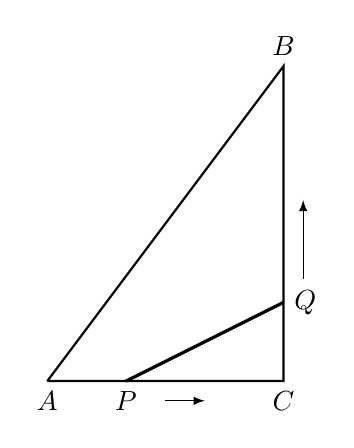
\begin{tikzpicture}[>=latex]
     \draw[thick] (0,0)node[below]{$A$}--(3,0)node[below]{$C$}--(3,4)node[above]{$B$}--(0,0) ;
     \draw[very thick] (1,0)node[below]{$P$}--(3,1)node[right]{$Q$};     
\draw [->] (1.5,-.25)--(2,-.25);
\draw [->] (3.25,1.3)--(3.25,2.3);
        \end{tikzpicture}
    \end{center}
    \caption{}
\end{figure}



\begin{solution}
设$P$、$Q$同时移动到$x$
秒时,$\triangle PCQ$的面积是8${\rm cm^2}$.由题意可知:
\[\frac{1}{2}\x 2x(6-x)=8\quad \Rightarrow\quad x^2-6x+8=0\]
$\therefore\quad x=\frac{6\pm\sqrt{36-32}}{2}=\frac{6\pm 2}{2}\quad\Rightarrow\quad x_1=4,\quad x_2=2$

经检验,两个解都符合题意.

答:$P$、$Q$两点同时由$A$、$C$出发,移动到2秒
时,或4秒时,$\triangle PCQ$的面积都等于8${\rm cm^2}$.
\end{solution}

\begin{example}
某生产队的粮食产量,两年内从60万斤增
加到79.35万斤,试问:平均每年增加百分之几?

\end{example}

\begin{solution}
设平均每年增加$x\%$, 则一年后的产量就是
$60(1+x\%)$万斤;两年后产量就应该是
$[60(1+x\%)](1+x\%)$万斤.

依题意可得:    
\[\begin{split}
    60(1+x\%)(1+x\%)&=79.35\\
60(1+x\%)^2&=79.35\\
(1+x\%)^2&=1.3225\\
1+x\%&=\pm 1.15\\
\frac{x}{100}&=\pm 1.15-1\\
x&=100(\pm 1.15-1)
\end{split}\]
$\therefore\quad x_1=15,\quad x_2=-215$

答:平均每年增加15\%.

这里讲的“平均每年增加的百分数”,通常都称
为“年增长率”.
\end{solution}

\begin{ex}
某工厂的产品,原来每件成本为300元,连续两次降低
成本后,现在每件成本为192元,如果两次降低成本的百分
数相同,求这个百分数.
\end{ex}




\begin{example}
一个容器内,装满了20升的纯酒精.第一
次倒出若干升以后,用水加满;第二次又倒出同样升
数的混合液,仍用水加满.这时,容器内还剩下5升
纯酒精.试求:第一次倒出多少纯酒精?
\end{example}

\begin{solution}
    设第一次倒出纯酒精$x$升.
则,加水以后,第二次倒出$x$升混合溶液
中,应含有纯酒精$\left(\frac{20-x}{20}\right)\cdot x$升.

依题意可以列出方程:
\[20-x-\left(\frac{20-x}{20}\right)x=5\]
整理后,得 $x^2-40x+300=0$

$\therefore\quad x=\frac{40\pm \sqrt{1600-1200}}{2}=\frac{40\pm 20}{2}\quad \Rightarrow\quad x_1=30,\quad x_2=10$

显然,$x_1=30$不符合题意,应舍去.

答:第一次倒出纯酒精10升.
\end{solution}

\begin{ex}
    试求例3.48中,第二次应倒出多少纯酒精?照这样倒下
去,再求一下第三次倒出多少纯酒精?
\end{ex}



\section*{习题3.4}
\addcontentsline{toc}{subsection}{习题3.4}

\begin{enumerate}
\item 一个数与自身的一半之积等于8,求这数.
\item 两个连续的奇数之积等于323,求这两奇数.
\item 两数之差为8,之积为128.求这两数之和.
\item 边长为10米的正方形,要使它的面积扩展到4倍.试
求:正方形的边长要增加多少?
\item 现有正方形、长方形各一个,长方形的宽比正方形的边
要短3cm,长方形的长却比正方形的边要多2cm.如果已知
长方形的面积是36${\rm cm}^2$,那么,正方形的边长、面积各应是
多少?
\item 从正方形木板上,锯下3cm宽的一个长方形,剩下的面
积是10${\rm cm}^2$.试求:正方形木板的面积是多少?
\item 有一张画的尺寸是12$\x$18(分米),要在它的四周镶上
一样宽的银边,如果银边的面积正好与画面相等.那么,银
边应当有多宽?
\item 如图3.13所示,把长方形铁皮的四个角,各剪去一个
边长为5cm的正方形,折
起四边,就可以做成一个
无盖盒子.如果这个盒子
的容积是1500${\rm cm}^3$,长
方形铁皮的长是宽的2倍.
那么,这块长方形长、宽
各多少?
\begin{figure}[htp]
    \centering
\begin{tikzpicture}[scale=.8]
\draw (0,0) rectangle (8,4);    
\draw [pattern=north east lines](0,0) rectangle (1,1);
\draw [pattern=north east lines](7,0) rectangle (8,1);
\draw [pattern=north east lines](0,3) rectangle (1,4);
\draw [pattern=north east lines](7,3) rectangle (8,4);
\draw [dashed](1,1) rectangle(7,3);
\end{tikzpicture}
    \caption{}
\end{figure}

\item 已知一圆半径为10cm, 而另有一小圆,它的面积等于已
知圆的一半.试求这小圆的半径.
\item 一家工厂,前年年产量是1500吨,今年年产量是3000
吨,试求:这家工厂这两年的平均增长率(百分数).(精
确到0.01).
\item 某车间一月份产值100万元,第一季度总产值350万元.
问:第一季度平均每月的产值增长百分之几?
\item 一个小组若干人,新年互送贺年片一张,已知全组共送
贺年片72张.问:这个小组应有几个人?
\item 一个容积为64升的容器,装满了纯酒精,第一次倒出若
干升以后,用水加满;第二次又倒出同样多的混合液后,用
水再加满.这时,经过鉴定,容器中含有水15升.试求:第
一次比第二次多倒出去多少纯酒精?
\end{enumerate}

\section*{本章内容要点}
一、学习一元二次方程所必要的预备知识和概
念:
\begin{enumerate}
    \item 完全平方公式:$(x\pm y)^2=x^2\pm 2xy+y^2$或
称为二数和(或差)的平方公式.当$x,y$取正数时,
这两个公式都可以用“画正方形”的方法加以验证.
\item 平方根的概念、性质及运算.

如果$x^2=a,\; (a\ge 0)$,那么$x$就是$a$的平方根,当
$a>0$时,它有两个平方根,记作$x=\pm\sqrt{a}$.当$a=0$
时,它有一个平方根,记作
$x=\sqrt{0}=0$.当$a<0$
时,它的平方根无意义.

正数的正平方根,叫做它的算术平方根,记作:
$x=\sqrt{a}\; (a>0)$.

零的算术根,仍然是0.

对于算术平方根
$x=\sqrt{a}\; (a\ge 0)$,有以下基本性
质:
\begin{enumerate}
    \item $(\sqrt{a})^2=a\qquad (a\ge 0)$
    \item $\sqrt{x^2}=|x|=\begin{cases}
        x& x\ge 0\\
        -x& x<0
    \end{cases}$
\end{enumerate}


算术平方根的运算法则:
\begin{enumerate}
    \item $\sqrt{a}\cdot \sqrt{b}=\sqrt{ab}\quad (a\ge 0,\; b\ge 0)$
    
    运用它,可以进行“因数移到根号里”和“因数
移到根号外”的变形.

\item $\frac{\sqrt{a}}{\sqrt{b}}=\sqrt{\frac{a}{b}}\quad (a\ge 0,\; b> 0)$

运用分数的基本性质及算术平方根的基本性质,
可以进行“有理化分母”的变形.

\item 把算术平方根化简(使被开方数的每个因数的
指数小于2;分母有理化)以后,相同被开方数的算
术根可以运用数系运算通性进行加、减运算.
\end{enumerate}

\item 求一个数的平方根,可以查平方根表,也可以
直接开平方,进行计算.
\item 实数.

无限不循环小数,称为无理数.例如:$\sqrt{2},\; -\sqrt{3},\; \pi,\; e,\; 0.01001000\cdots$,等都是无理数.

无理数与有理数,统称为实数.

任一个非零实数$a$, 都有一个相反数$-a$, 且满足
$a+(-a)=0$; 都有一个倒数$\frac{1}{a}$,
且满足$a\cdot \frac{1}{a}=1$.

实数的运算,同样具有运算通性.
\end{enumerate}

\vskip 2ex 
二、一元二次方程的标准式是
$$ax^2+bx+c=0\qquad (a\ne 0)$$
它的解法有:

\begin{enumerate}
    \item 配方法:关键是先化为二次项系数为1的形
式,然后将方程“两边加上一次项系数一半的平方
数”,使方程一边成为完全平方形式.
\[\begin{split}
    x^2+\frac{b}{a}x+\frac{c}{a}&=0\\
    x^2+\frac{b}{a}x+\left(\frac{b}{2a}\right)^2&=\left(\frac{b}{2a}\right)^2-\frac{c}{a}\\
    \left(x+\frac{b}{2a}\right)^2&=\frac{b^2-4ac}{4a^2}
\end{split}\]
\begin{equation}
    x=\frac{-b\pm\sqrt{b^2-4ac}}{2a}
\end{equation}

\item 公式法——把方程化为标准式,找出各项系数
$a,b,c$,代入(3.4)就可以求出根.
\item 换元法——如果能把方程整理成如下形式
\[a(x+m)^2+b(x+m)+c=0\qquad (a\ne 0)\]
那么,可以设$(x+m)=y$, 原方程化为
\[ay^2+by+c=0\qquad  (a\ne 0)\]
用求根公式先求出$y$的值,然后再代入原设:$(x+m)
=y$, 进而求出原方程的根.
\item 对于$b=0$, 或$c=0$, 或$b=c=0$时的特殊一元
二次方程,除以上一般解法外,还可以直接运用数系
运算通性(特别是分配律)、平方根的意义等方法,
求出方程的根.
\end{enumerate}

\vskip 2ex 
三、利用一元二次方程,还可以解一些特殊的高
次方程,其主要方程是换元法——设辅助未知数.通
过换元,把高次转化为低次方程,从而可以由已知解
法的低次方程,逐步达到求出未知的高次方程的根.
本章我们所遇到过的有以下几种形式:
\begin{enumerate}
    \item $ ax^4+bx^2+c=0\qquad  (a\ne 0)$
    
    可设$x^2=y$, 原方程化为$ay^2+by+c=0$.
    \item $a(mx^2+nx)^2+b(mx^2+nx)+c=0\qquad  (a\ne 0)$
    
    可设$mx^2+nx=y$, 原方程化为$ay^2+by+c=0$.
    \item $a(mx^2+nx+p)(mx^2+nx+q)+b=0$
    
    可设$mx^2+nx=y$, 原方程化为$a(y+p)(y+q)+b=0$.
    \item $ax^3+bx^2+cx=0\qquad (a\ne 0)$
    
    用分配律:$(ax^2+bx+c)x=0$,把原方程可以
化为两个低次方程求解,即:
$ax^2+bx+c=0$ 或 $x=0$
\end{enumerate}

\vskip 2ex 
四、一元二次方程根的判别式:
\[\Delta =b^2-4ac\]
这是判别任一个一元二次方程的根是否存在以及存在
什么样的实数根的准绳.即
\begin{enumerate}
\item 当$\Delta>0$时,$ax^2+bx+c=0$有两不等实根.
\item 当$\Delta=0$时,$ax^2+bx+c=0$有两相等实根(重
根).
\item 当$\Delta<0$时,$ax^2+bx+c=0$无实数根.
\end{enumerate}

五、用一元二次方程解应用问题,其方法与主要
步骤与第二章一次方程解应用题是一样的.其要点仍
是:弄清题意,分析量与量之间的关系,引入未知
数,列出方程式,这是解决问题的基础;进而解方
程,得到实数解(或无解).这是解决问题的关键;
最后,还应检验所得解是否符合题意.舍去不合理
的,留下符合题意的,写出答案.


\section*{复习题三}
\addcontentsline{toc}{section}{复习题三}
\begin{enumerate}
    \item 利用和的平方公式,你能推导出和的立方公式吗?即
    \[(a+b)^3=(a+b)^2\cdot (a+b)\]
    \item 用开平方方法,计算以下算术平方根:
    $$\sqrt{0.7744},\qquad \sqrt{9880.36},\qquad \sqrt{100.4004}$$
  \item 
    \begin{enumerate}
        \item 正方形的面积是55225${\rm m^2}$,试求它的边长是
多少?
\item 长方体的体积是7500${\rm cm^2}$,长、宽、高的比
是$5:4:3$. 试求长方体的长、宽、高各是多少?
    \end{enumerate}
    
    
\item 查表并计算:(用四位平方根表)
\begin{enumerate}
    \item $\sqrt{82340}-\sqrt{8234}$
    \item $\sqrt{376.8}+\sqrt{37.68} -\sqrt{3.678}$
\end{enumerate}

\item 举例说明:
\begin{enumerate}
    \item 在无理数范围内,加、减、乘、除四则运算是“不
封闭”的.
\item 在实数范围内,开方运算并不是通行无阻的.
\end{enumerate}

\item $x,y$取什么样的实数时,下列各式才能成为恒等式:
\begin{multicols}{2}
    \begin{enumerate}
        \item $\frac{\sqrt{x^2}}{x}=1$
        \item $\frac{\sqrt{x^2}}{x}=-1$
        \item $\frac{|y|}{y}=1$
        \item $\frac{\sqrt{y^2}}{|y|}=1$
        \item $|x-1|+\sqrt{y-2}=0$
    \end{enumerate}
\end{multicols}



\item 一个数的多少倍的平方根,才能等于它的平方根的10
倍?
\item 一个正方形的面积增大为原来的2倍时,它的边长增大
为原边长的多少倍?面积要增大3倍时,边长增大几倍?这
样推下去,正方形的面积增大$n$倍时,边长增加几倍?
\item $x$取什么值时,下列算术平方根有意义:
\[\sqrt{1-x},\qquad \sqrt{x-2}\cdot \sqrt{x},\qquad \sqrt{(x-3)^2}  \]

\item 试决定下列各算式的符号:
\begin{enumerate}
    \item $\frac{\sqrt{2}}{2}-\frac{\sqrt{3}}{3}$
    \item $\sqrt{(5-a)^2}-\sqrt{(a-5)^2} \quad (a>5)$
\end{enumerate}

\item 计算:
\begin{enumerate}
    \item $\sqrt{45}-\frac{1}{5}\sqrt{5}-\frac{1}{3}\sqrt{20}$
    \item $\frac{3\sqrt{6}}{2\sqrt{3}}-\sqrt{128}+2\sqrt{\frac{1}{2}}$
    \item $5\sqrt{24}-3\sqrt{1\frac{1}{2}}-\sqrt{54}-\sqrt{24}$
    \item $\frac{\sqrt{8}}{\sqrt{5}\cdot \sqrt{6}}$
    \item $\left(4\sqrt{3}-3\right)\left(3\sqrt{2}+5\sqrt{3}\right)-1$
    \item $\frac{\sqrt{5}+\sqrt{6}}{\sqrt{3}}+\frac{2\sqrt{3}-5\sqrt{10}}{\sqrt{5}}$
    \item $\left(6\sqrt{\frac{3}{2}}-3\sqrt{\frac{1}{2}}\right)-\left(3\sqrt{\frac{2}{3}}-\frac{1}{3}\sqrt{18}\right)$
    \item $\sqrt{\frac{1}{2}}+\sqrt{45}-\sqrt{12.5}-0.5\sqrt{200}+\sqrt{242}+6\sqrt{1\frac{1}{8}}-\sqrt{245}$
\end{enumerate}

\item 计算:
\begin{enumerate}
    \item $\left(5\sqrt{5}-5\right)^2-\left(5\sqrt{5}-1\right)^2$
    \item $\frac{12-\sqrt{3}}{2\sqrt{6}}-\sqrt{6}+\left(5\sqrt{3}-3\sqrt{8}\right)^2$
    \item $\left(\frac{-1-\sqrt{3}}{2}\right)^2-\left(\frac{-1+\sqrt{3}}{2}\right)^2$
    \item $\left(\frac{1}{2}\sqrt{\frac{1}{2}}-\frac{3}{2}\sqrt{\frac{1}{3}}+\frac{5}{4}\sqrt{\frac{4}{5}}\right)\div \frac{8}{15}\sqrt{\frac{1}{8}}$

\end{enumerate}

\item 先配方,再证明:
\begin{enumerate}
    \item $x$取任何实数时,$x^2+12x+40$总是正值.
    \item $x$取任何实数时,$x^2-16x+65$总不小于1.
\end{enumerate}

\item 解下列一元二次方程:
\begin{enumerate}
    \item $2x^2+3x-1=0$
    \item $2t^2+1=4t$
    \item $\frac{3}{2}y^2+4y=1$
    \item $x^2+6000x-4\x 10^7=0$
    \item $(x+1)(x-1)=2\sqrt{2}x$
    \item $\left(\frac{x}{a}-1\right)^2=\left(\frac{x}{b}+1\right)^2\quad (a^2\ne b^2)$
    \item $\frac{1}{2}\left\{\frac{1}{2}\left[\frac{1}{2}\left(\frac{1}{2}x^2+2\right)+2\right]+2\right\}=2$
    \item $x-7+\frac{(x-6)^2}{2}=\frac{(x+4)^2}{2}-\frac{(x+2)(x+6)}{2}$
\end{enumerate}

\item 解下列方程:
\begin{enumerate}
    \item $x^2-2ax=m^2$
    \item $mx^2+1=x+m\quad (m>\frac{1}{2})$
    \item $(x+a)(x-a)=1$
    \item $x^2-ax-bx+\frac{a^2}{4}+\frac{b^2}{4}=0$
\end{enumerate}

\item 用换元法解下列高次方程:
\begin{enumerate}
    \item $x^4-6x^2=0$
    \item $2x^4-19x^2+9=0$
    \item $\sqrt{3}(x^2-x)^2=\sqrt{2}(x^2-x)$
    \item $(6x^2-7x)^2-2(6x^2-7x)-3=0$
    \item $(2x^2-1)^4-(2x^2-1)^2=0$
    \item $x\left(x-\sqrt{3}\right)\left(x-2\sqrt{3}\right)\left(x-3\sqrt{3}\right)=216$
    \item $(x^2+5x+4)(x^2+5x+6)-120=0$
\end{enumerate}

\item 已知一元二次方程
$7x^2+mx+n=0$有两个根$2$, $-\frac{3}{7}$,
试求$m,n$的值.

\item $x$取何值时,
\begin{enumerate}
    \item $x^2-6x+5$的值等于0?
    \item $x^2-6x+5$的值等于$-4$?
    \item $x^2-6x+5$的值与$x+1$的值相等?
\end{enumerate}

\item $m$取何值时,
\begin{enumerate}
    \item 方程$3x^2-2(3m+1)x+3m^2-1=0$有一个根是0?
    \item 方程$3x^2-2(3m+1)x+3m^2-1=0$能有重根?
\end{enumerate}

\item $k$为何值时,
\begin{enumerate}
    \item 方程$kx^2-12x+4=0$有重根?
    \item 方程$(a+2)x^2-2akx+k=0$有重根?
($a$为已知数且$a\ne-2$).
\end{enumerate}

\item 已知方程$x^2-ax+2a=0$的一个根是1,
\begin{enumerate}
    \item 试求$a$的值,
    \item 求另一个根.
\end{enumerate}

\item 已知方程$ax^2+bx+c=0$与方程$x^2-1=0$有一个公共
根,试求:$a,b,c$之间的关系.
\item 已知方程$2x^2+2(a+b)x+a^2+b^2=0$有重根,且$a,b$
为实数,求证:$a=b$.
\item 今有四个连续整数,已知其中最小的数与其中最大的
数之积等于这四个数之和,试求这四个数.
\item 数字和是8的两位数,乘以它的两位数字交换位置后
所得的另一个两位数,等于1855.试求这个两位数.
\item 有一个长方形场地,长比宽多4米.现在要环绕这个
长方形四周,修建一条宽2米的道路,使这条环形道所占的
面积与这个场地的面积相等.试求:这个长方形场地的面
积.
\item 要在长2.4m,宽2m的长方形中间,挖去一块面积是
1.92${\rm m^2}$的小长方形,使剩下的长方环形四周都一样宽.
试求这个宽度?
\item 甲、乙两块长方形地里,共植树416棵,甲地比乙地多
植树196棵,如果两块地里所植树木的排数都是比行数少1.
试求:甲、乙两块地里各种几排,几行?
\item 20公升纯酒精正好装满一个木桶,倒出若干公升以
后,用水加满;再倒出同样多的混合液以后,再用水加满.
这时,木桶中的水正好是全桶的$\frac{3}{4}$.

试求:第一次、第二次
各倒出纯酒精多少公升?
\item 试试看:
\begin{enumerate}
    \item 把一元二次方程$ax^2+bx+c=0\; (a\ne 0)$的两个根(在
    $b^2-4ac\ge 0$时)相加,你能得到什么结论?举例验证你的结
论.
\item 再把两根相乘,又能得到什么结论?再举 例验证你
    的结论.
\end{enumerate}

\item 试求$p,q$为何值时,一元二次方程
$x^2+px+q=0$的根也等于$p$和$q$?

提示:由于
\[\begin{cases}
    p^2+p^2+q=0\\
    q^2+pq+q=0
\end{cases}\]
即:
\begin{numcases}{}
    q=-2p^2\\
    q(q+p+1)=0
\end{numcases}
将(3.5)代入(3.6)得:$p^2(2p^2-p-1)=0$.

解出$p$的值代入(3.5),可求出相应的$q$值.

经检验,得:$p_1=0,\quad q_1=0,\quad p_2=1,\quad q_2=-2$

还有$p_3=-\frac{1}{2},\quad q_3=-\frac{1}{2}$,
但不符合题意,应舍去.

\end{enumerate}

